% $Header: /cvsroot/latex-beamer/latex-beamer/solutions/conference-talks/conference-ornate-20min.en.tex,v 1.6 2004/10/07 20:53:08 tantau Exp $

\documentclass{beamer}

\mode<presentation>
{
%  \usetheme{Hannover}
\usetheme[width=0.7in]{Hannover}
% or ...

  \setbeamercovered{transparent}
  % or whatever (possibly just delete it)
}
\usepackage{longtable}
\usepackage{booktabs}
\usepackage{qtree}

\usepackage[english]{babel}
% or whatever

\usepackage[latin1]{inputenc}
% or whatever

\usepackage{times}
%\usepackage[T1]{fontenc}
% Or whatever. Note that the encoding and the font should match. If T1
% does not look nice, try deleting the line with the fontenc.
%\usepackage{logictheme}

\usepackage{multirow}
\usepackage{totpages}
\usepackage{hyperref}
\usepackage{booktabs}
\usepackage[round]{natbib}

\usepackage{listings}
\lstset{frame=none, showstringspaces=false, basicstyle=\ttfamily\footnotesize,
  xleftmargin=-8mm,language=Haskell}

\usepackage{tikz}
\usetikzlibrary{positioning}

\usepackage{pifont}
\usepackage{amsmath,amsfonts,xspace,xcolor,url}
\newcommand{\cross}{\ding{55}}

\newcommand{\blt}{- } %used for bullets in a list

\newcounter{datadefnum} %Datadefinition Number
\newcommand{\ddthedatadefnum}{DD\thedatadefnum}
\newcommand{\ddref}[1]{DD\ref{#1}}

\newcommand{\colAwidth}{0.1\textwidth}
\newcommand{\colBwidth}{0.8\textwidth}

\renewcommand{\arraystretch}{1.1} %so that tables with equations do not look crowded

\pgfdeclareimage[height=0.7cm]{logo}{McMasterLogo}
\title[\pgfuseimage{logo}] % (optional, use only with long paper titles)
{The Drasil Framework for Literate Scientific Software}

%\subtitle
%{Include Only If Paper Has a Subtitle}

\author[Slide \thepage~of \pageref{TotPages}] % (optional, use only with lots of
                                              % authors)
{\textbf{Spencer Smith}, Jacques Carette, Dan Szymczak, Steven Palmer}
% - Give the names in the same order as the appear in the paper.
% - Use the \inst{?} command only if the authors have different
%   affiliation.

\institute[McMaster University] % (optional, but mostly needed)
{
  Computing and Software Department\\
  Faculty of Engineering\\
  McMaster University
}
% - Use the \inst command only if there are several affiliations.
% - Keep it simple, no one is interested in your street address.

\date[Jan 12, 2016] % (optional, should be abbreviation of conference name)
{CSE/SHARCNET Seminar in Scientific Computing, November 23, 2016}
% - Either use conference name or its abbreviation.
% - Not really informative to the audience, more for people (including
%   yourself) who are reading the slides online

\subject{computational science and engineering, software engineering, software
  quality, literate programming, software requirements specification, document
  driven design}
% This is only inserted into the PDF information catalog. Can be left
% out. 

% If you have a file called "university-logo-filename.xxx", where xxx
% is a graphic format that can be processed by latex or pdflatex,
% resp., then you can add a logo as follows:

%\pgfdeclareimage[height=0.5cm]{Mac-logo}{McMasterLogo}
%\logo{\pgfuseimage{Mac-logo}}

% Delete this, if you do not want the table of contents to pop up at
% the beginning of each subsection:
% \AtBeginSubsection[]
% {
%   \begin{frame}<beamer>
%     \frametitle{Outline}
%     \tableofcontents[currentsection,currentsubsection]
%   \end{frame}
% }

% If you wish to uncover everything in a step-wise fashion, uncomment
% the following command: 

%\beamerdefaultoverlayspecification{<+->}

\beamertemplatenavigationsymbolsempty 

% have SRS and LP open during the presentation

\begin{document}

%%%%%%%%%%%%%%%%%%%%%%%%%%%%%%%%%%%%%%
\hoffset=-.4in %removing side bar for these frames
\begin{frame}[plain]

\titlepage

\end{frame}
\hoffset=0in %restore
%%%%%%%%%%%%%%%%%%%%%%%%%%%%%%%%%%%%%%

% \begin{frame}

% \frametitle{Literate Scientific Software}
% \tableofcontents
% % You might wish to add the option [pausesections]

% % make like a story - the phases - reason for, why works, advantages
% % changing the history a bit to make a more rational narrative

% \end{frame}

%%%%%%%%%%%%%%%%%%%%%%%%%%%%%%%%%%%%%%

\begin{frame}

\frametitle{Abstract}

\begin{itemize}
\item \textbf{Goal} -- Improve quality of SCS
\item \textbf{Idea} -- Adapt ideas from SE
\item \textbf{Document Driven Design}
\begin{itemize}
\item Good -- improves quality
\item Bad -- ``manual'' approach is too much work
\end{itemize}
\item \textbf{Solution}
\begin{itemize}
\item Capture knowledge
\item Generate all things
\item Traceability
\end{itemize}
\item \textbf{Showing great promise}
\begin{itemize}
\item Significant work yet to do
\item Looking for examples/partners
\end{itemize}
\end{itemize}

\end{frame}

%%%%%%%%%%%%%%%%%%%%%%%%%%%%%%%%%%%%%%

\section[Scope]{Scope}

%%%%%%%%%%%%%%%%%%%%%%%%%%%%%%%%%%%%%%

\hoffset=-.8in
\begin{frame}[plain, fragile]

\frametitle{Scope: Large/Multiyear} %replace with pictures

\begin{tikzpicture}[remember picture,overlay]
\node [xshift=0cm,yshift=0.15cm] at (current page.center)
{
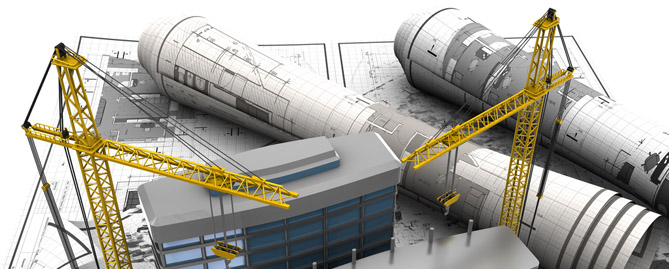
\includegraphics[width=1.15\textwidth]{MSc_CE.jpg}
};
\end{tikzpicture}

\end{frame}
\hoffset=0in

%%%%%%%%%%%%%%%%%%%%%%%%%%%%%%%%%%%%%%

\hoffset=-.8in
\begin{frame}[plain, fragile]

\frametitle{Scope: Program Families}

% if time add another program family example

\begin{tikzpicture}[remember picture,overlay]
\node [xshift=0cm,yshift=-3.cm] at (current page.center)
{
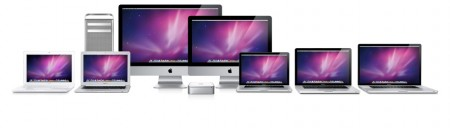
\includegraphics[width=1.2\textwidth]{apple-mac-products-450x128.jpg}
};
\end{tikzpicture}

\begin{tikzpicture}[remember picture,overlay]
\node [xshift=0cm,yshift=1.cm] at (current page.center)
{
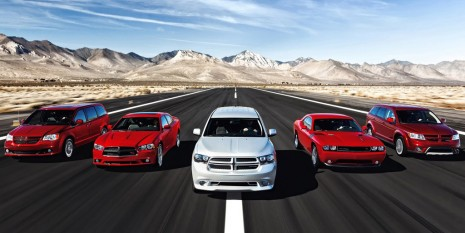
\includegraphics[width=0.8\textwidth]{dodge-lineup.jpg}
};
\end{tikzpicture}

\end{frame}
\hoffset=0in

%%%%%%%%%%%%%%%%%%%%%%%%%%%%%%%%%%%%%%

\hoffset=-.8in
\begin{frame}[plain, fragile]

\frametitle{Scope: End User Developers} 
% end user developers solving physics problems

\begin{tikzpicture}[remember picture,overlay]
\node [xshift=0cm,yshift=-0.2cm] at (current page.center)
{
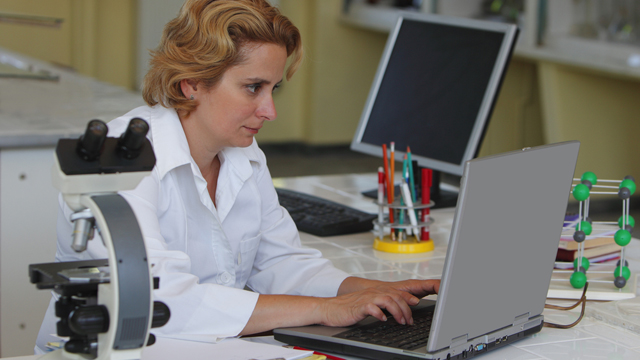
\includegraphics[width=1\textwidth]{ScientistAtAComputer.jpg}
};
\end{tikzpicture}

\end{frame}
\hoffset=0in

%%%%%%%%%%%%%%%%%%%%%%%%%%%%%%%%%%%%%%

\hoffset=-.8in
\begin{frame}[plain, fragile]

\frametitle{Scope: Physical Science} %replace with pictures

\begin{tikzpicture}[remember picture,overlay]
\node [xshift=3.75cm,yshift=0.9cm] at (current page.center)
{
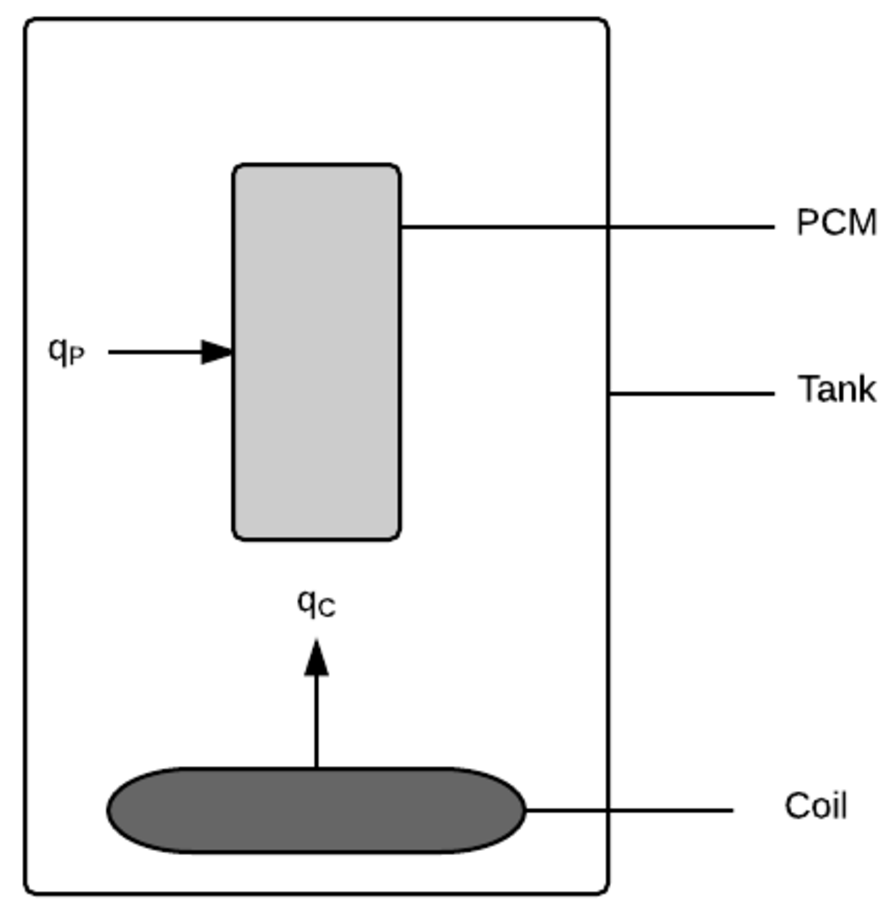
\includegraphics[width=0.4\textwidth]{Tank.pdf}
};
\end{tikzpicture}

\begin{tikzpicture}[remember picture,overlay]
\node [xshift=-3.5cm,yshift=1.55cm] at (current page.center)
{
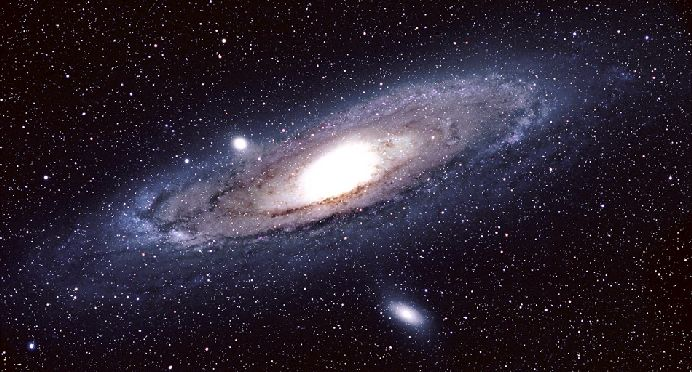
\includegraphics[width=0.5\textwidth]{m31_jg.jpg}
};
\end{tikzpicture}

\begin{tikzpicture}[remember picture,overlay]
\node [xshift=0.1cm,yshift=0.8cm] at (current page.center)
{
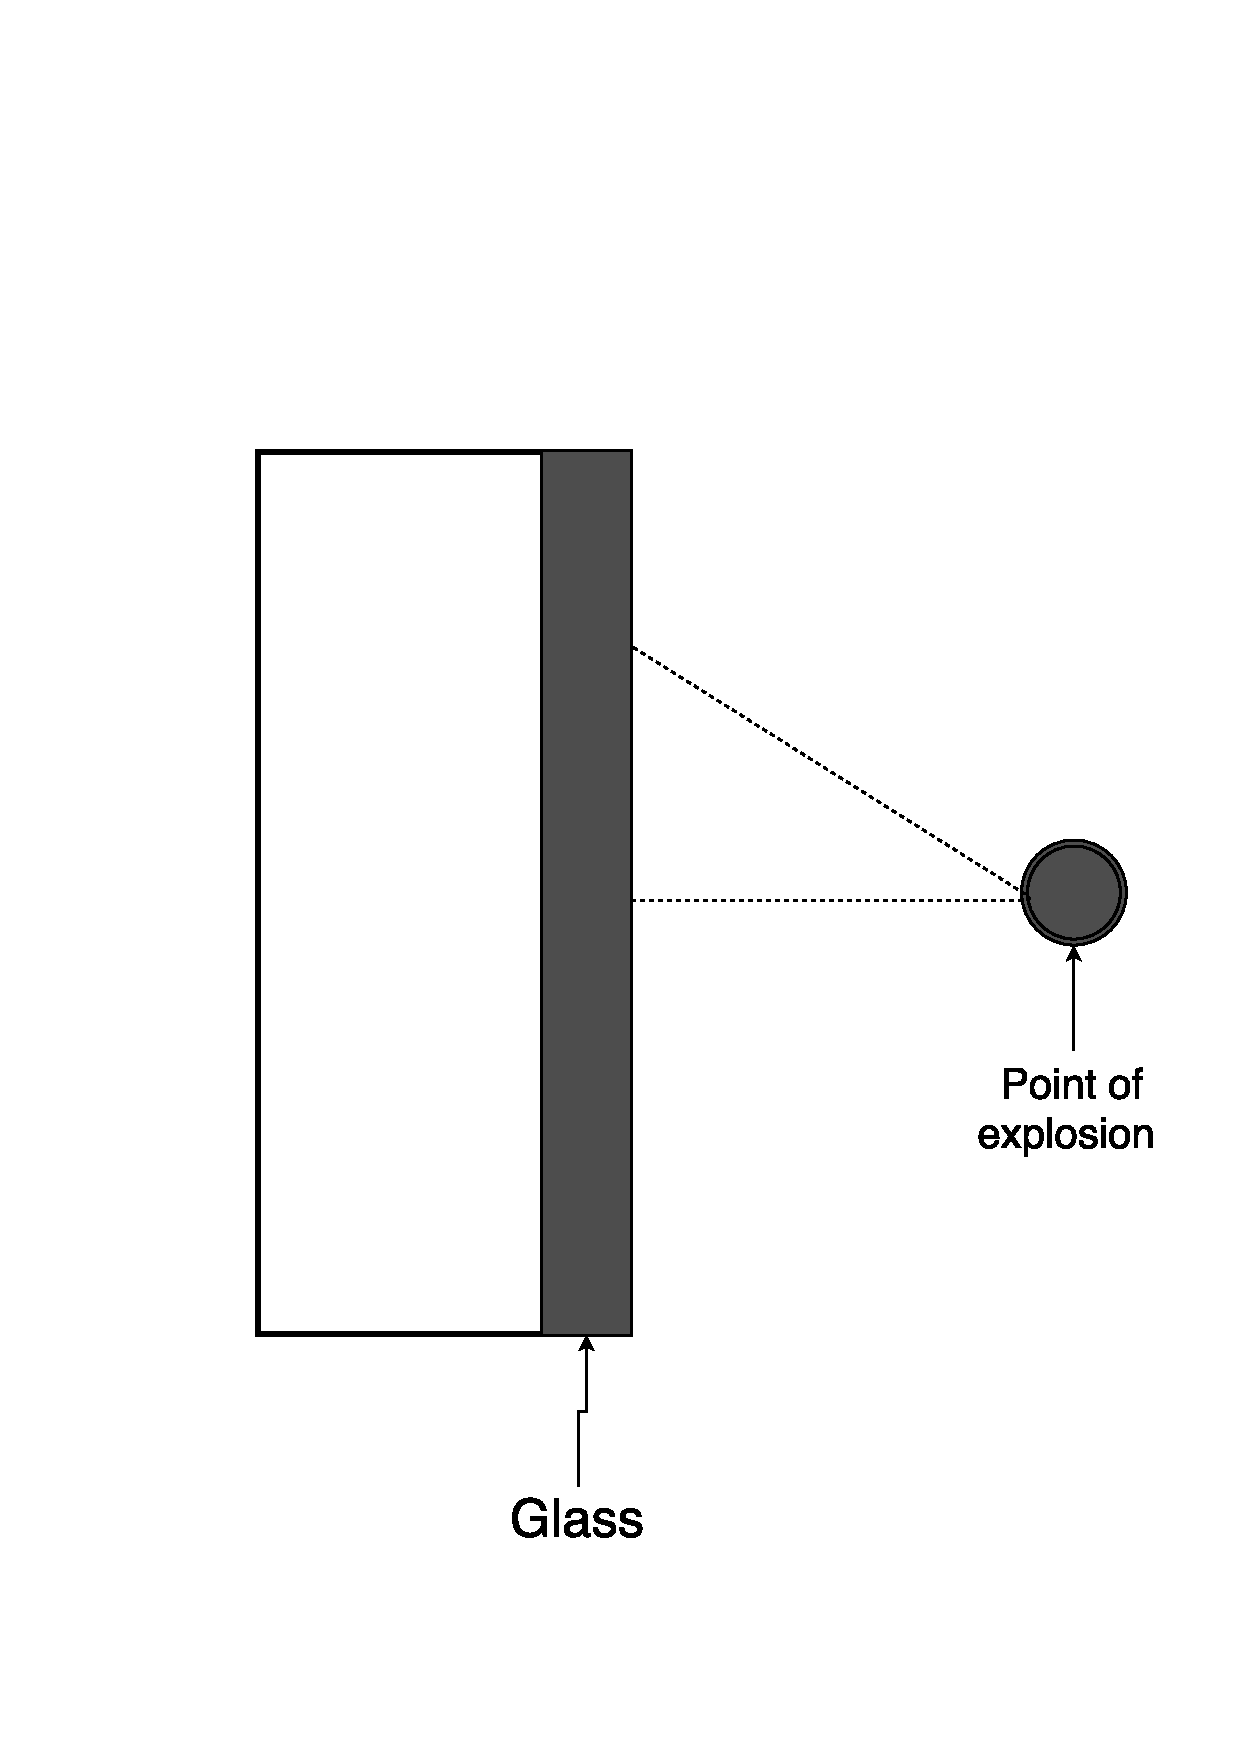
\includegraphics[width=0.3\textwidth]{physicalsystimage.pdf}
};
\end{tikzpicture}

\begin{tikzpicture}[remember picture,overlay]
\node [xshift=-3.5cm,yshift=-2.25cm] at (current page.center)
{
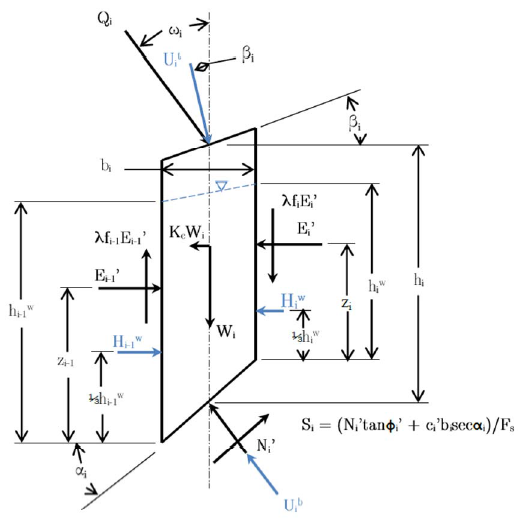
\includegraphics[width=0.4\textwidth]{ForceDiagram.png}
};
\end{tikzpicture}

\begin{tikzpicture}[remember picture,overlay]
\node [xshift=0.5cm,yshift=-2.75cm] at (current page.center)
{
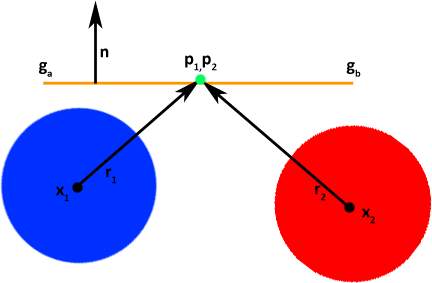
\includegraphics[width=0.3\textwidth]{grooveJoint.png}
};
\end{tikzpicture}

\begin{tikzpicture}[remember picture,overlay]
\node [xshift=4.25cm,yshift=-2.75cm] at (current page.center)
{
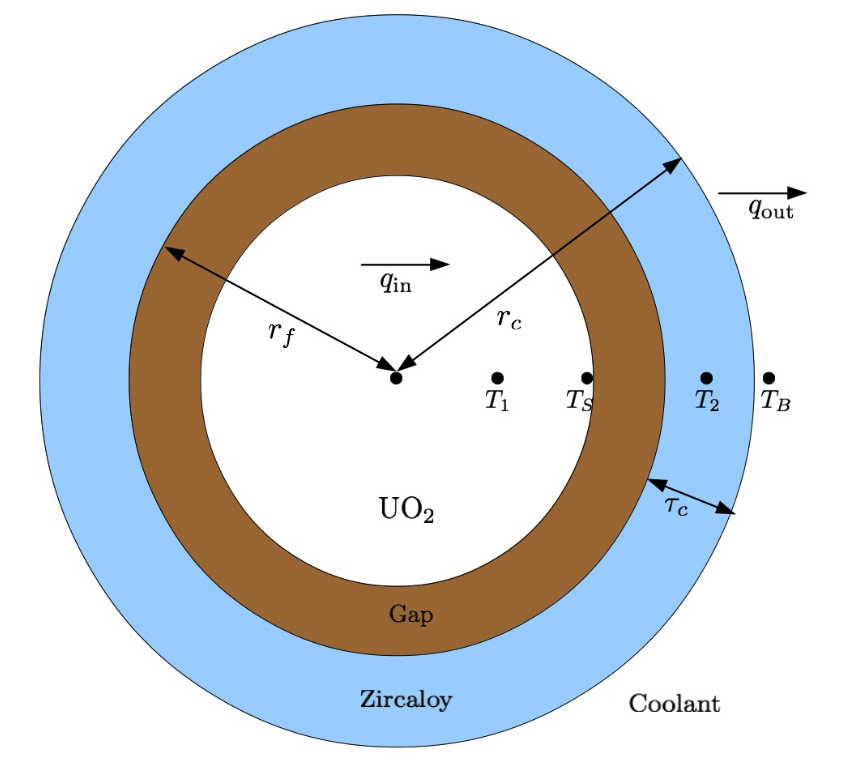
\includegraphics[width=0.3\textwidth]{fuelpin.png}
};
\end{tikzpicture}

\end{frame}
\hoffset=0in

%%%%%%%%%%%%%%%%%%%%%%%%%%%%%%%%%%%%%%

\section[Motivation]{Motivation}

%%%%%%%%%%%%%%%%%%%%%%%%%%%%%%%%%%%%%%

\hoffset=-.8in
\begin{frame}[plain, fragile]

\frametitle{Motivation: Safety}

% picture of reactor, MRI

\begin{tikzpicture}[remember picture,overlay]
\node [xshift=-0.1cm,yshift=0.75cm] at (current page.center)
{
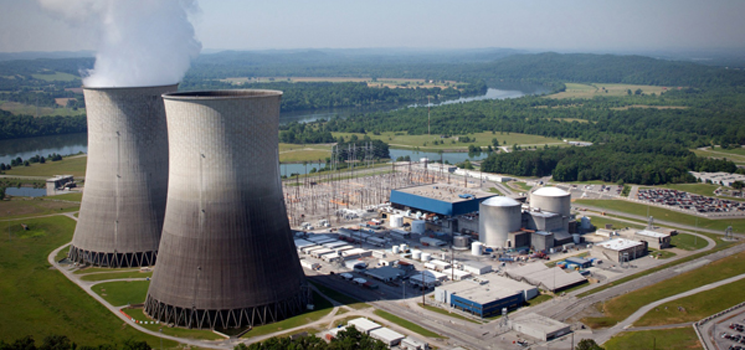
\includegraphics[width=1.1\textwidth]{nuclear_reactor_technologies_home.png}
};
\end{tikzpicture}

\begin{tikzpicture}[remember picture,overlay]
\node [xshift=1.75cm,yshift=-1.75cm] at (current page.center)
{
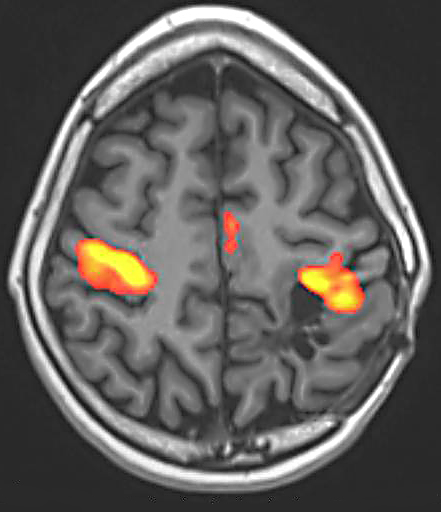
\includegraphics[width=0.4\textwidth]{fmri-image.jpg}
};
\end{tikzpicture}

\end{frame}
\hoffset=0in

%%%%%%%%%%%%%%%%%%%%%%%%%%%%%%%%%%%%%%

\hoffset=-.8in
\begin{frame}[plain, fragile]

\frametitle{Motivation: (Re)certification}

% picture of stamp

\begin{tikzpicture}[remember picture,overlay]
\node [xshift=0cm,yshift=0cm] at (current page.center)
{

\includegraphics[width=0.8\textwidth]{certified.jpg}
};
\end{tikzpicture}

\end{frame}
\hoffset=0in

%%%%%%%%%%%%%%%%%%%%%%%%%%%%%%%%%%%%%%

\begin{frame}

\frametitle{Motivation: Improve Quality}

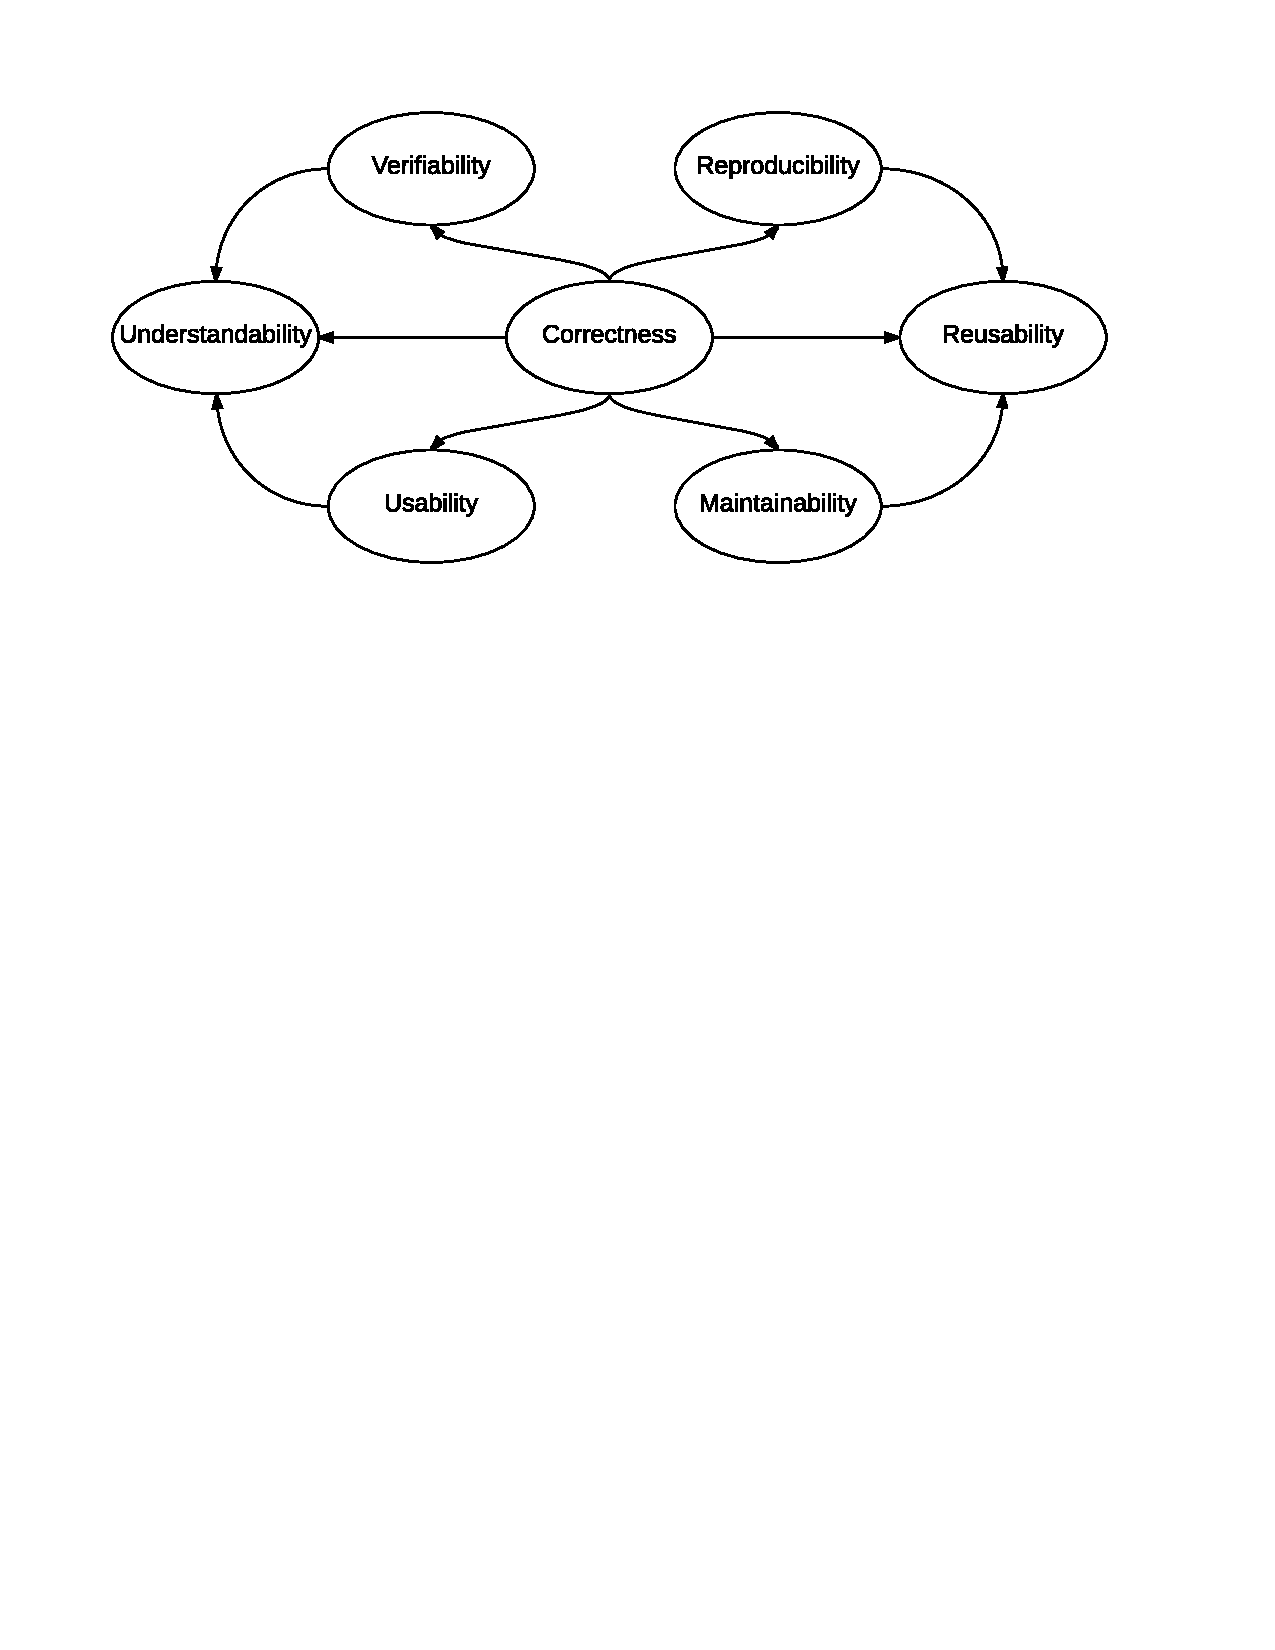
\includegraphics[width=1\textwidth]{RelationBWQualities.pdf}

\end{frame}

%%%%%%%%%%%%%%%%%%%%%%%%%%%%%%%%%%%%%%

\section[Curr.\ Approach]{Current Approach to Developing SCS}

%%%%%%%%%%%%%%%%%%%%%%%%%%%%%%%%%%%%%%

\begin{frame}

\frametitle{Current Approach}

\begin{itemize}
\item Agile like \citep{CarverEtAl2007}
\item Amethododical \citep{Kelly2013}
\item Knowledge acquisition driven \citep{Kelly2015}
\item Each stage reports counterproductive \citep{Roache1998}
\item Limited tool use \citep{Wilson2006}
\item Limited testing of code \citep{KellyAndSanders2008a}
\item Lack of understanding of testing \citep{Merali2010}
\item Missed opportunities for reuse \citep{Owen1998} 
 %-- 37 of 52 triangular mesh generators
 % implemented the same triangulation algorithm
\item Emphasis on:
\begin{enumerate}
\item Science~\citep{Kelly2007}
\item Code
\end{enumerate}
\end{itemize}

\end{frame}

%%%%%%%%%%%%%%%%%%%%%%%%%%%%%%%%%%%%%%

% \begin{frame}

% \frametitle{Challenges for DDD}

% \begin{itemize}
% \item Up front requirements
% \item Rapid change for numerical algorithms
% \item Information duplication
% \item Synchronization headaches between artifacts
% \item Perceived over-emphasis on non-executable artifacts
% %Parnas paper - people do not like docs, vicious cycle
% \end{itemize}

% \end{frame}

%%%%%%%%%%%%%%%%%%%%%%%%%%%%%%%%%%%%%%

\section[DDD]{Document Driven Design}

%%%%%%%%%%%%%%%%%%%%%%%%%%%%%%%%%%%%%%

\begin{frame}

\frametitle{``Faked'' Rational Design Process}

\begin{center}
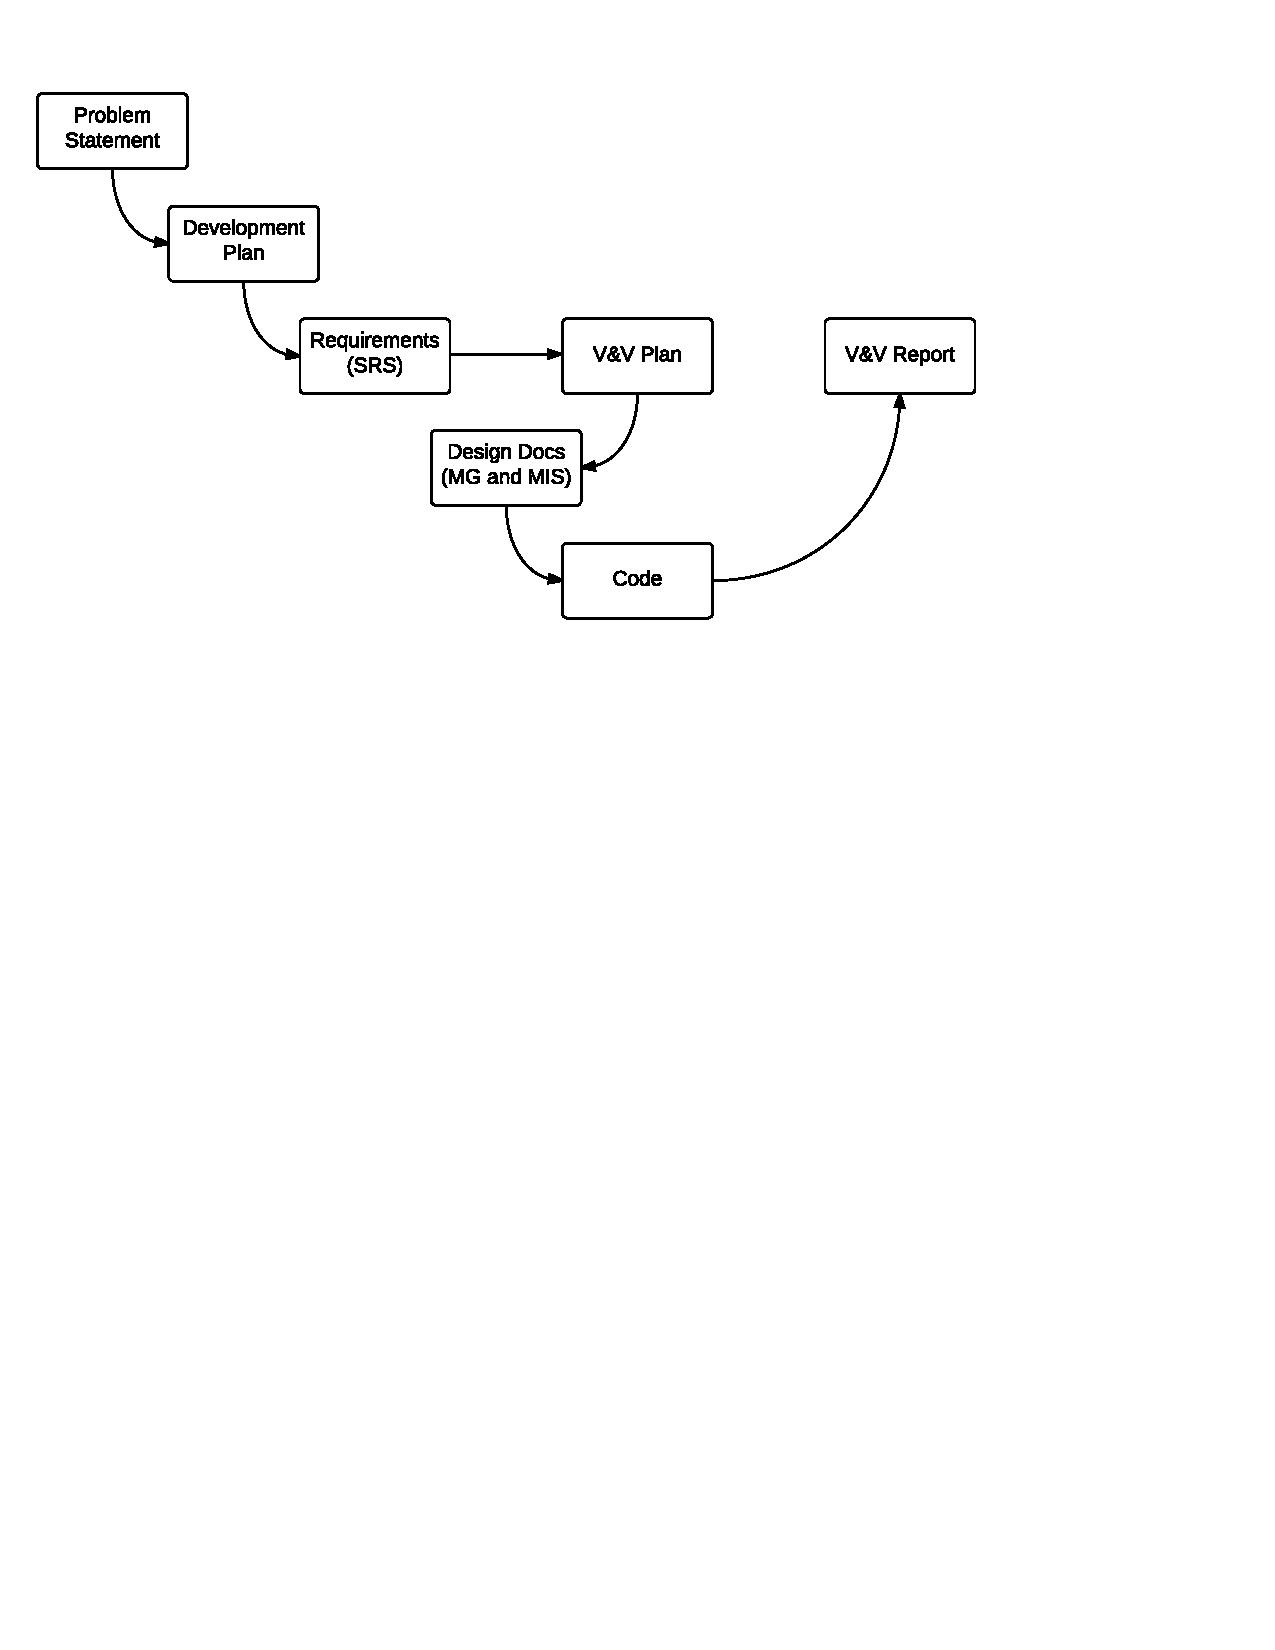
\includegraphics[scale=0.6]{OverviewOfProcess.pdf}
\end{center}

SWHS example at
\href{https://github.com/smiths/swhs}{https://github.com/smiths/swhs}

\end{frame}

%%%%%%%%%%%%%%%%%%%%%%%%%%%%%%%%%%%%%%

% \begin{frame}

% \frametitle{Solar Water Heating Tank}

% \begin{center}
% 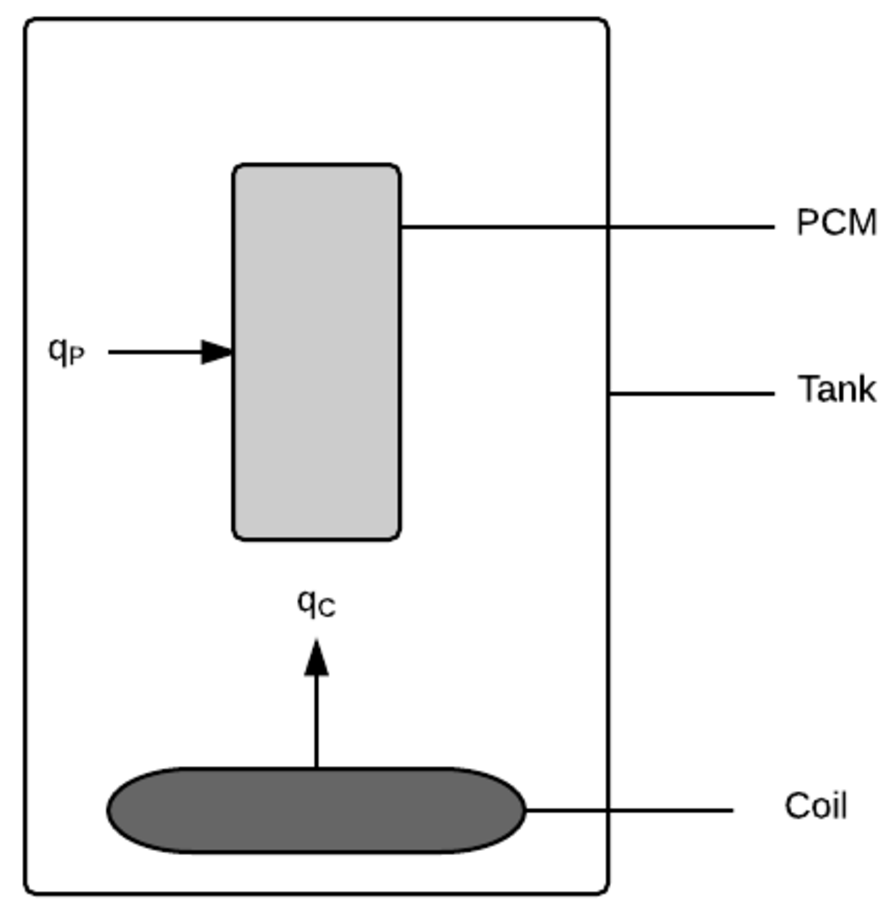
\includegraphics[scale=0.45]{Tank.pdf}
% \end{center}

% \href{https://github.com/smiths/swhs}{https://github.com/smiths/swhs}

% \end{frame}

%%%%%%%%%%%%%%%%%%%%%%%%%%%%%%%%%%%%%%

\hoffset=-.4in %removing side bar for these frames

\begin{frame}[plain, fragile]

%\frametitle{SRS for SWHS}

\begin{center}
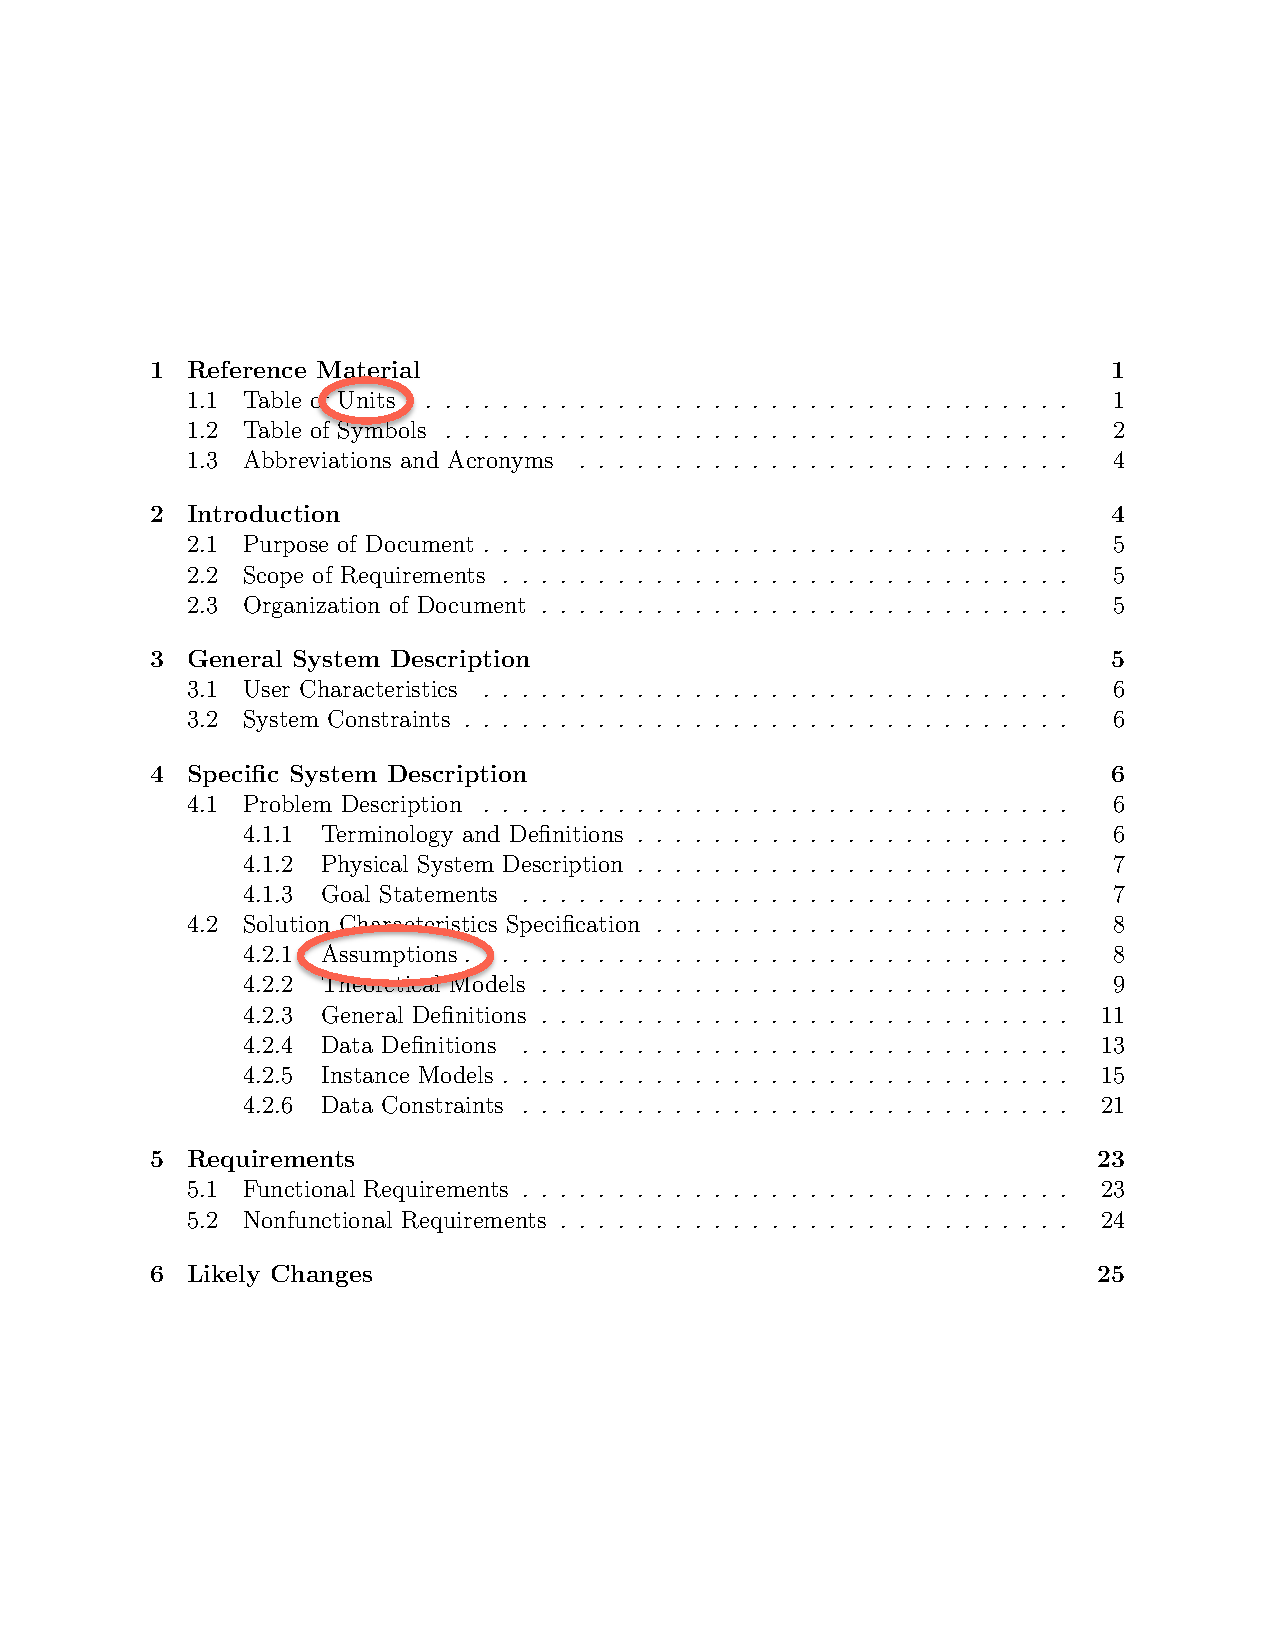
\includegraphics[scale=0.55]{TofC.pdf}
\end{center}

\end{frame}
\hoffset=0in

%%%%%%%%%%%%%%%%%%%%%%%%%%%%%%%%%%%%%%

\begin{frame}

\frametitle{Reusability}

\noindent
\begin{minipage}{\columnwidth}
\begin{tabular}{@{} p{\colAwidth}  p{\colBwidth}@{}}
\toprule
\textbf{Num.}& \textbf{T1} \\
\midrule
Label &\bf Conservation of energy\\
\midrule
Eq &  $-{\bf \nabla \cdot q} +q'''$ = $\rho C \frac{\partial T}{\partial t}$ \smallskip\\
\midrule
Descrip & The above equation gives the conservation of energy for time 
varying heat transfer in a material of specific heat capacity $C$ and density $\rho$,
where $\bf q$ is the thermal flux vector, $q'''$ is the volumetric heat
generation, $T$ is the temperature, $\nabla$ is the del operator and $t$ is the time.\\
\bottomrule
\end{tabular}
\end{minipage}

\end{frame}

%%%%%%%%%%%%%%%%%%%%%%%%%%%%%%%%%%%%%%

\begin{frame}

\frametitle{Maintainability}

\begin{itemize}

\item[A1:] The
  only form of energy that is relevant for this problem is thermal energy.  All
  other forms of energy, such as mechanical energy, are assumed to be
  negligible [T1].

\item[A2:] All heat transfer coefficients are constant over time [GD1].

\item[A3:] The water in
  the tank is fully mixed, so the temperature is the same throughout the entire
  tank [GD2, DD2].

\item[A4:] The PCM has the same temperature throughout [GD2, DD2, LC1].

\item[A5:] etc.

\end{itemize}

\end{frame}

%%%%%%%%%%%%%%%%%%%%%%%%%%%%%%%%%%%%%%

\hoffset=-.7in %removing side bar for these frames

\begin{frame}[plain, fragile]

\frametitle{SWHS Traceability Graph}

\begin{center}
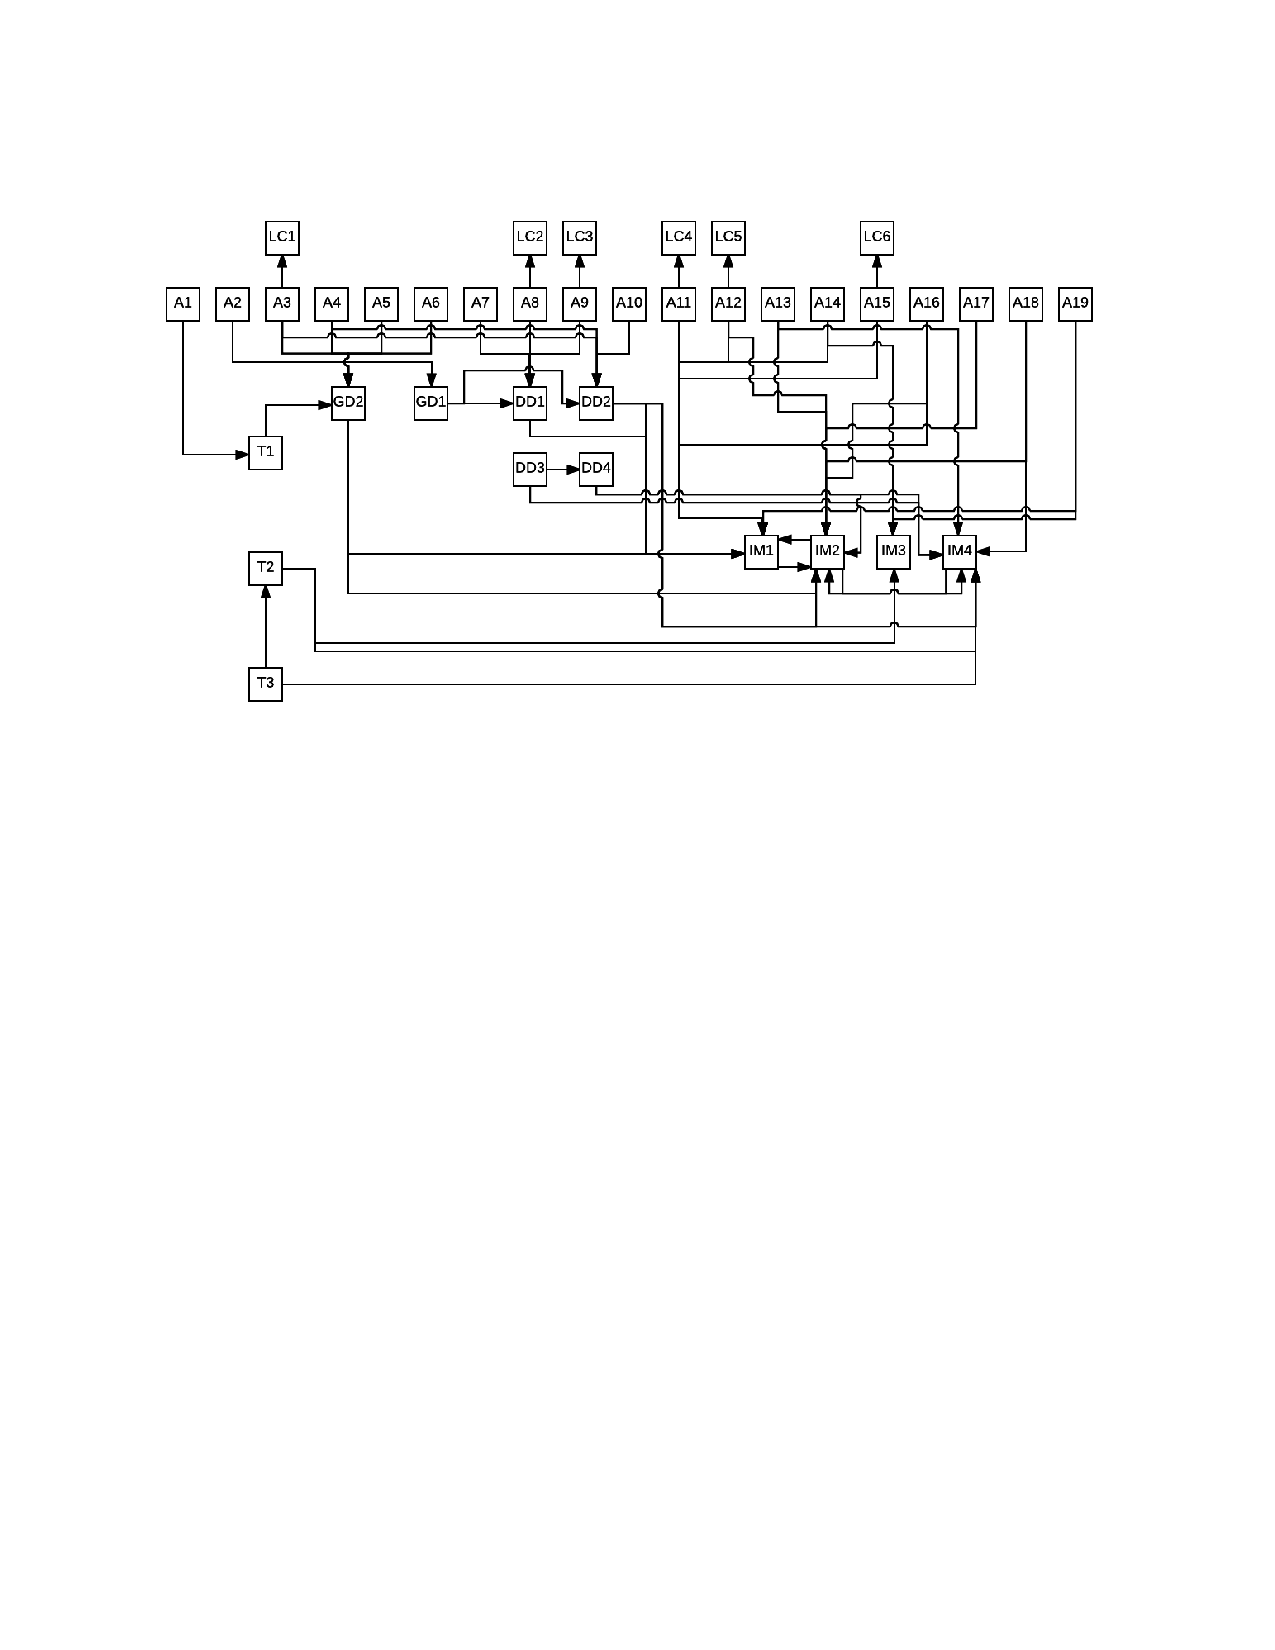
\includegraphics[scale=0.75]{TraceGraph.pdf}
\end{center}

\end{frame}
\hoffset=0in
%%%%%%%%%%%%%%%%%%%%%%%%%%%%%%%%%%%%%%

\begin{frame}

\frametitle{Verifiability}

\begin{table} 
\centering
%\caption{Constraints on quantities}
\begin{tabular}{c c r c } 
\toprule
\textbf{Var} & \textbf{Constraints} & \textbf{Typical Value} & \textbf{Uncertainty}\\ \midrule
$L$ & $L > 0$ & 1.5 m & 10\% \\ 
$D$ & $D > 0$ & 0.412 m & 10\% \\ 
$V_P$ & $V_P > 0$ & 0.05 m$^3$	& 10\% \\
$A_P$ & $A_P > 0$ & 1.2 m$^2$	& 10\% \\
$\rho_P$ & $\rho_P > 0$	& 1007 kg/m$^3$	& 10\% \\
\bottomrule
\end{tabular}
\label{tab:pcm}
\end{table}

\begin{equation*}
E_W = \int_{0}^{t} h_C A_C (T_C - T_W(t)) dt - \int_{0}^{t} h_P A_P (T_W(t) - T_P(t)) dt
\end{equation*}

% \begin{itemize}
% \item Sanity checks captured and reused
% \item Generate guards against invalid input
% \item Generate test cases
% \end{itemize}
\end{frame}

%%%%%%%%%%%%%%%%%%%%%%%%%%%%%%%%%%%%%%

\begin{frame}

\frametitle{Reproducibility}

\cite{IonescuAndJansson2013} show reproducibility challenges due to
undocumented:
\begin{itemize}
\item Assumptions
\item Modifications
\item Hacks
\end{itemize}

% \begin{itemize}
% \item Knowledge is explicitly stored for the future
% \item Recipes used to regenerate all artifacts, not just code or results
% \item Recipes include build instructions
% \end{itemize}
\end{frame}

%%%%%%%%%%%%%%%%%%%%%%%%%%%%%%%%%%%%%%

\begin{frame}

\frametitle{Complete Documentation}

\noindent
\begin{minipage}{\columnwidth}
\begin{tabular}{@{} p{\colAwidth}  p{\colBwidth}@{}}
\toprule
% \textbf{Number}& \textbf{IM2} \\
% \midrule
% Label & \bf Energy balance on PCM to find $T_P$\\
% \midrule
Input&  $m_P$, $C_P^S$, $C_P^L$, $h_P$, $A_P$, $t_\text{final}$, $T_\text{init}$, $T_\text{melt}^P$,
$T_W(t)$ from IM1\\
\midrule
Output & $T_P(t)$, $0 \leq t \leq t_\text{final}$, with initial 
conditions, $T_W(0) = T_P(0) = T_\text{init}$ (A12), and $T_W(t)$ 
from IM1, such that the following governing ODE is satisfied.  The
specific ODE depends on $T_P$ as follows:\\
&  $
  \frac{dT_P}{dt} = \begin{cases}
  \frac{dT_P}{dt} = \frac{1}{\tau^S_P}(T_W(t) - T_P(t)) & \text { if } T_P<T_\text{melt}^P\\
  \frac{dT_P}{dt} = \frac{1}{\tau^L_P}(T_W(t) - T_P(t)) & \text { if } T_P>T_\text{melt}^P\\
  0 & \text { if }  T_P=T_\text{melt}^P \\
   ~ & \text{ and } 0 < \phi < 1\\
  \end{cases}
  $
\\
\bottomrule
\end{tabular}
\end{minipage}

\end{frame}

%%%%%%%%%%%%%%%%%%%%%%%%%%%%%%%%%%%%%%

\hoffset=-.7in %removing side bar for these frames

\begin{frame}[plain, fragile]

\frametitle{SWHS Uses Hierarchy}

\begin{center}
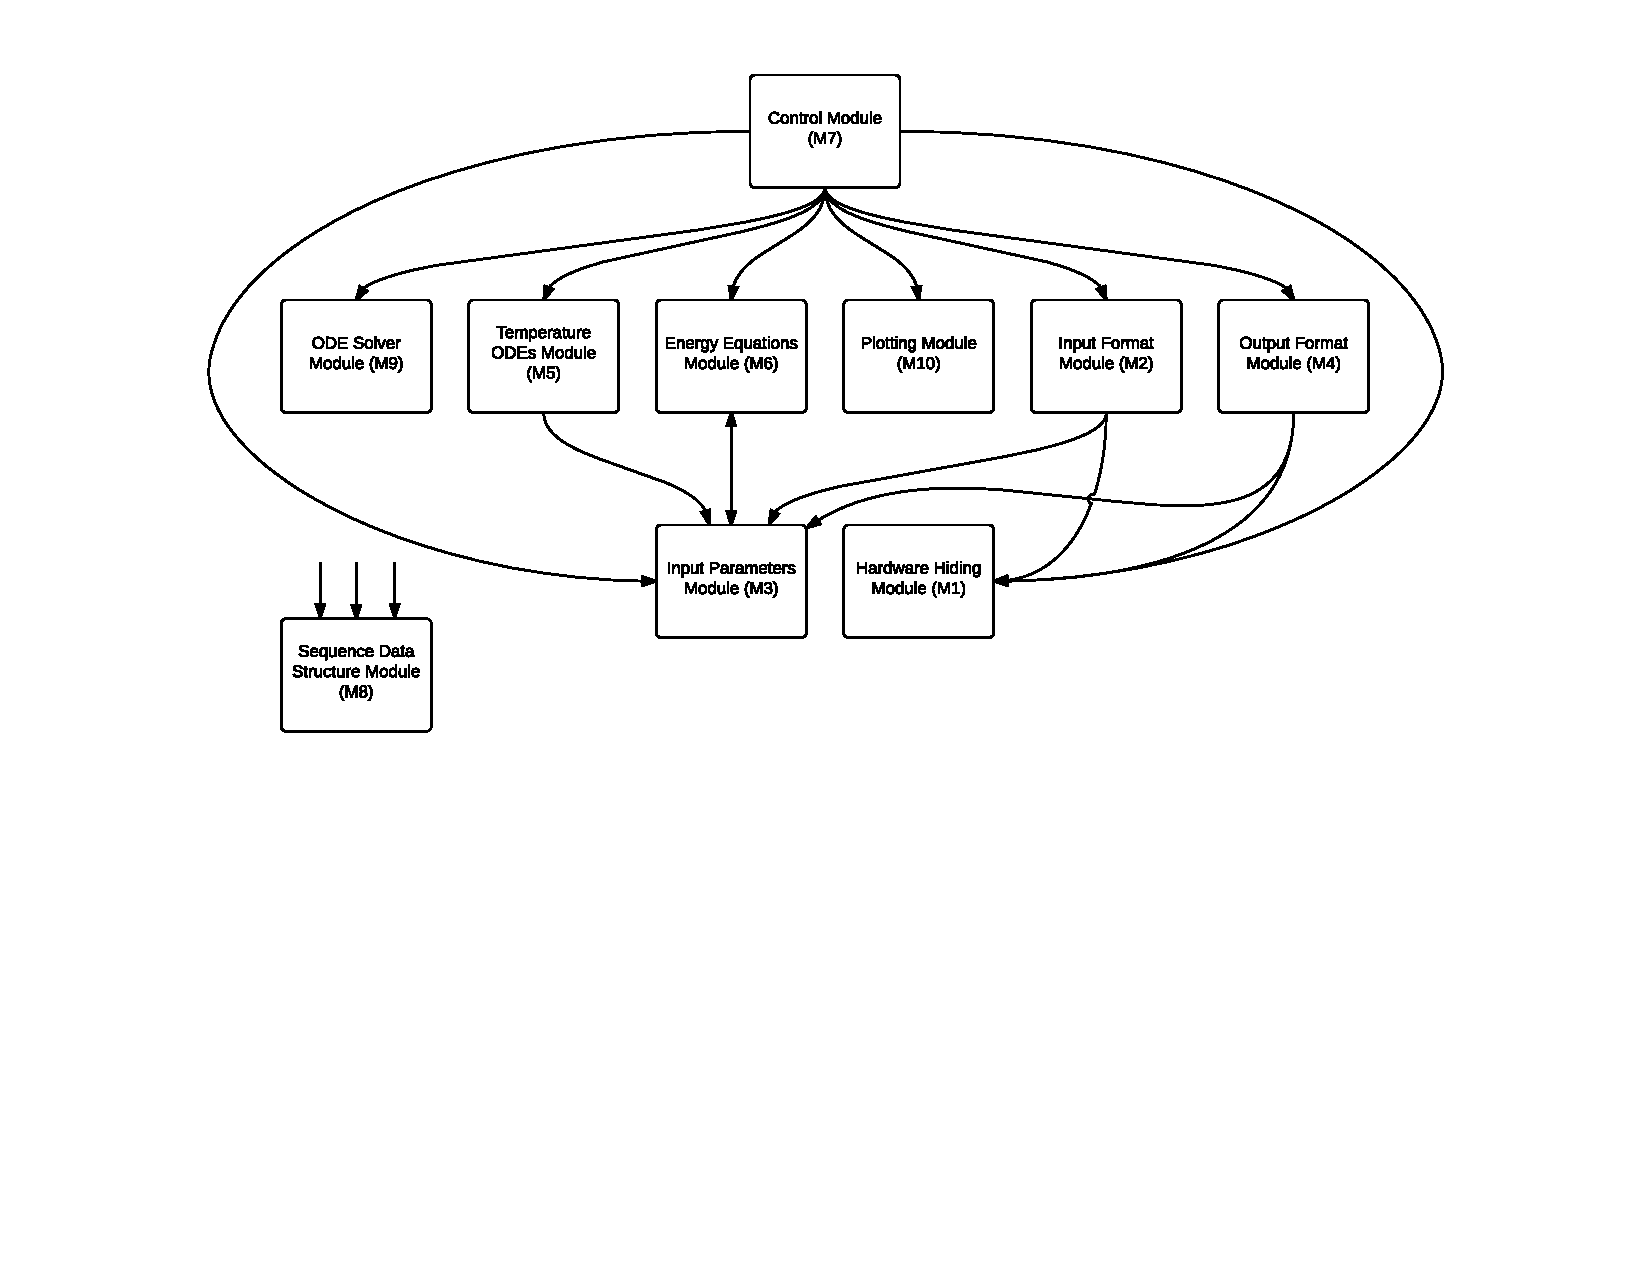
\includegraphics[scale=0.57]{UsesHierarchy.pdf}
\end{center}

\end{frame}
\hoffset=0in

%%%%%%%%%%%%%%%%%%%%%%%%%%%%%%%%%%%%%%

\begin{frame}

\frametitle{Verification and Validation}

\begin{itemize}
\item Compare to closed-form solutions
\item Method of manufactured solutions
\item Interval arithmetic
\item Convergence studies
\item Compare to another program
\item Mutation testing
\item Metamorphic testing
\item Code inspections
\end{itemize}

\end{frame}

%%%%%%%%%%%%%%%%%%%%%%%%%%%%%%%%%%%%%%

\begin{frame}

\frametitle{Tools and Development Practices}

\begin{itemize}
\item Unit Testing
\item Version control
\item Issue tracking
\item Performance measurement
\item Virtual machines
\item Follow best practices \citep{WilsonEtAl2014}
\end{itemize}

\end{frame}

%%%%%%%%%%%%%%%%%%%%%%%%%%%%%%%%%%%%%%

\begin{frame}[plain]

\frametitle{Literate Programming}

\hspace{-2.3cm}
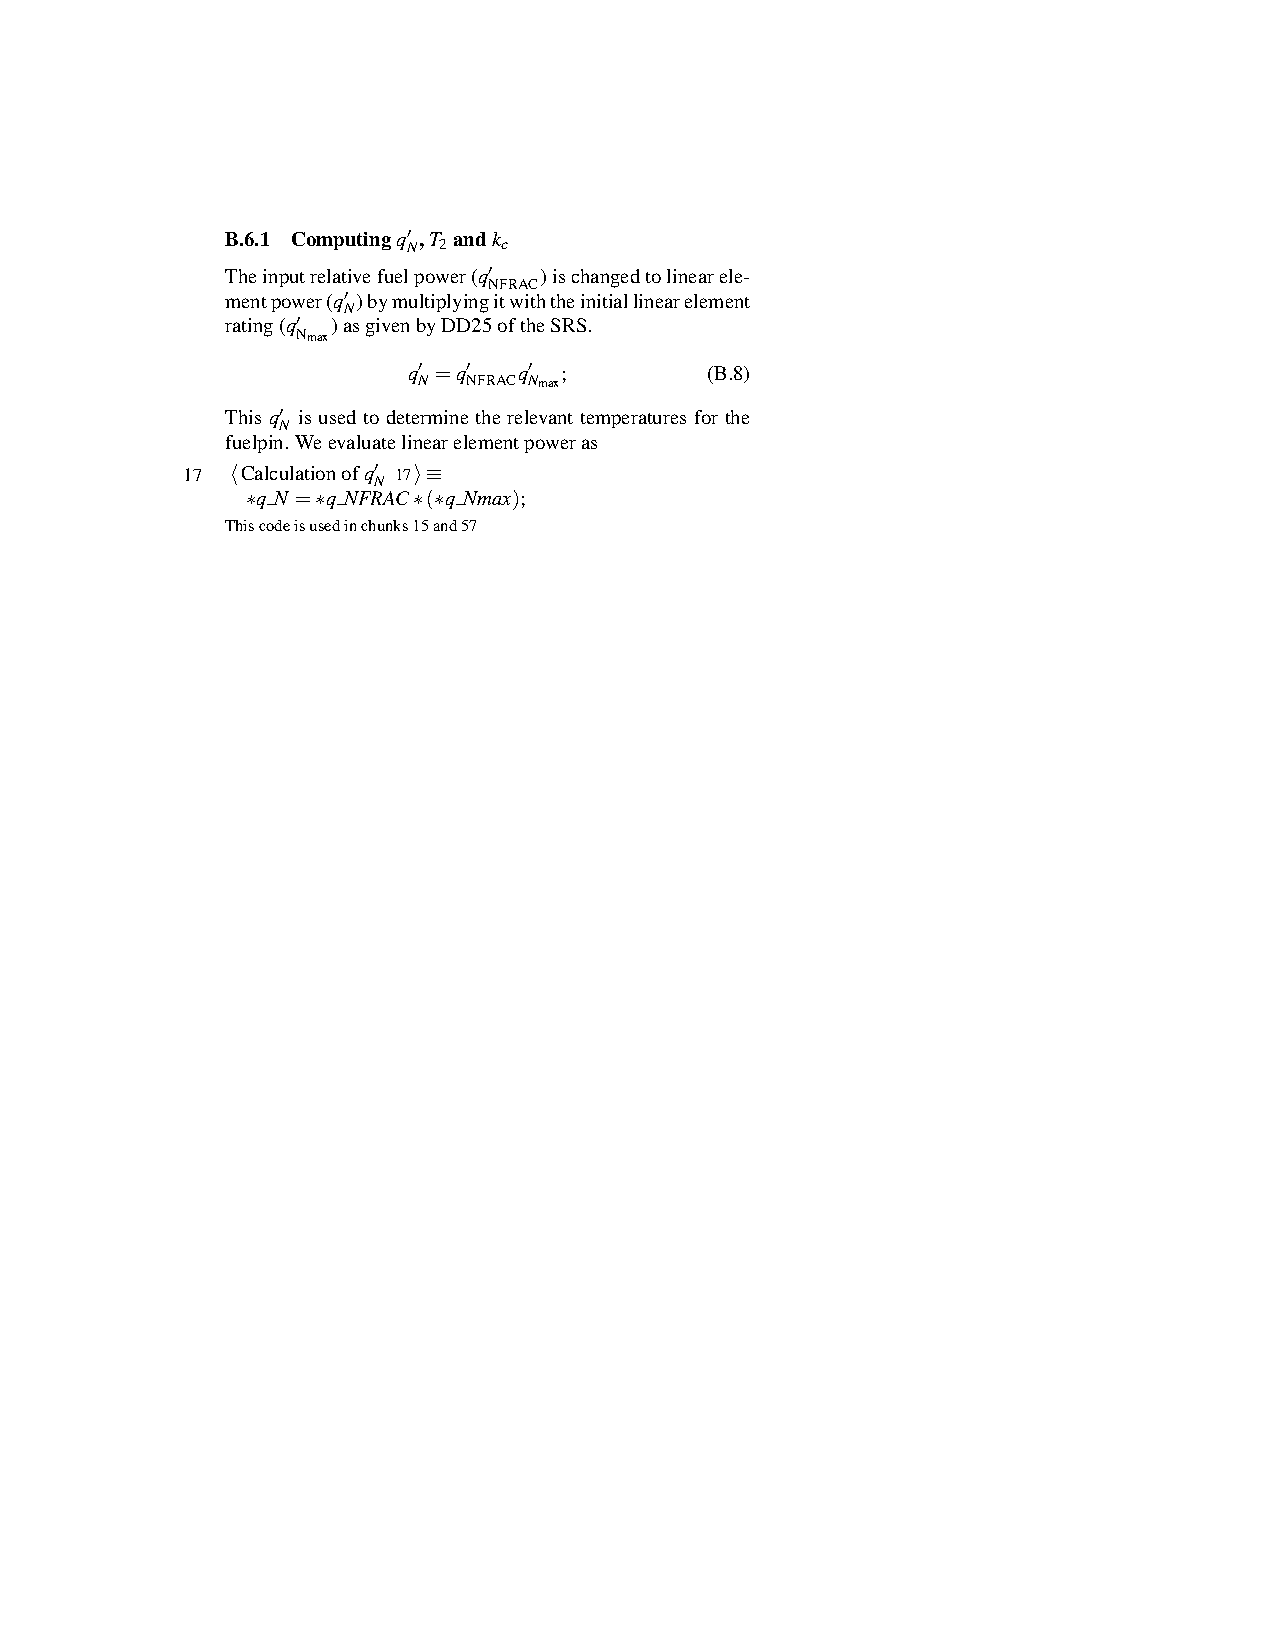
\includegraphics[width=1.22\columnwidth]{qnfrac.pdf}

\end{frame}

%%%%%%%%%%%%%%%%%%%%%%%%%%%%%%%%%%%%%%

\subsection[Advantages]{Advantages}

%%%%%%%%%%%%%%%%%%%%%%%%%%%%%%%%%%%%%%

\begin{frame}[fragile]

\frametitle{\citet{SmithAndKoothoor2016}}

\begin{align}
R_1^{\mathrm{code}} &= \frac{f}{8\pi k_{\mathrm{AV}}} + \frac{1}{2\pi r_f h_g} \\
 R_1^{\mathrm{manual}} & = \frac {f}{8 \pi k_{\mathrm{AV}}}+ \frac{1}{2\pi r_f h_g}+\frac{\tau_c}{4\pi r_f k_c}
\end{align}

%actually equiv is hg is replaced with hp in the manual equation, since hg
%includes hg and kc
 
\begin{itemize}
\item Uncovered 27 issues with the previous documentation
\begin{itemize}
\item Incompleteness ($R_{\mbox{gap}}$)
\item Inconsistency($r$, $r_0$, $h_g$)
\item Verifiability problems ($R_1$)
\item Lack of traceability (circuit analogy)
\end{itemize}
\item Advantages of proposed approach
\begin{itemize}
\item Abstract to concrete
\item Separation of concerns
%\item Table of Symbols, unique labels, cross-referencing, and consistency checks
\item Every equation, assumption, definition, model, derivation, source and
  traceability between them
%\item Checklist.
\end{itemize}
\end{itemize}

\end{frame}

%%%%%%%%%%%%%%%%%%%%%%%%%%%%%%%%%%%%%%

\begin{frame}

\frametitle{\citet{SmithJegatheesanAndKelly2016}}

\begin{enumerate}

\item Select 5 small to medium size SCS
\item Interview code owners
\item Redevelop using DDD
\item Interview code owners
\item Analyze responses

\end{enumerate}

\end{frame}

%%%%%%%%%%%%%%%%%%%%%%%%%%%%%%%%%%%%%%

\hoffset=-.6in %removing side bar for these frames

\begin{frame}[plain, fragile]

\frametitle{Summary of Case Studies}

  \begin{tabular}{lrlclccccc}
    \toprule
    & \textbf{LOC} & \textbf{Lng} & \textbf{ND} & \textbf{Age} 
    & \textbf{SE} & \textbf{Prg} & \textbf{Tst} & \textbf{VC} & \textbf{Bug}\\

    \midrule \textbf{SWHS} & 1000 & F77 & 1 & 5 & \cross &
                                                           \checkmark
                                 & \cross & \cross & \cross \\
	  
    \textbf{Astro} &5000 & C & 2 & 10 & \ding{55} &
                                                             \checkmark & \cross & \cross & \cross \\
      
    \textbf{Glass} & 1300 & F90 & 1 & $<$1 & \cross &
                                                               \checkmark & \cross & \cross & \cross \\

    \textbf{Soil} & 800 &  M & 1 & 5 & \checkmark &
                                                             \checkmark & \checkmark & \checkmark & \cross \\
	  
    \textbf{Neuro} & 1000 & M & 1 & 5 & \checkmark &
                                                              \checkmark & \cross & \checkmark & \cross \\
	  
    \textbf{Acoust} & 200 & M & 4 & 2.5 & \cross &
                                                            \checkmark & \cross & \cross & \cross \\
	  		
    \bottomrule
				
  \end{tabular}  

\end{frame}
\hoffset=0in %resetting side bar

%%%%%%%%%%%%%%%%%%%%%%%%%%%%%%%%%%%%%%

\begin{frame}

\frametitle{Advantages}

\begin{itemize}
%\item Add Parnas advantages?
\item \structure{Documentation of assumptions}
\item \structure{All variables have explicit units}
\item SRS helpful with new graduate students
\item Modules result in more user friendly code
\item \structure{Traceability between modules and requirements useful}
\item Better organized code
\item Information sharing on design choices
\item \structure{Detailed record of knowledge capital}
\item Code is produced to make testing easier
\end{itemize}

\end{frame}

%%%%%%%%%%%%%%%%%%%%%%%%%%%%%%%%%%%%%%

\subsection[Disadvantages]{Disadvantages}

%%%%%%%%%%%%%%%%%%%%%%%%%%%%%%%%%%%%%%

\begin{frame}

\frametitle{Disadvantages (Perceived and Real)}

\begin{itemize}
\item \structure{SRS is too long}
\item SRS is not necessary
\item DDD will not work in reality, since \structure{needs upfront requirements}
\item \structure{Too much SE jargon}
%\item \structure{Uses hierarchy in MG unclear}
\item Difficult without a team of people
\end{itemize}

\end{frame}

%%%%%%%%%%%%%%%%%%%%%%%%%%%%%%%%%%%%%%

\begin{frame}

\frametitle{Information Duplication}
\begin{center}
\includegraphics[width=.6\textwidth]{Copies.jpg}
\end{center}
\begin{itemize}
%\item Reduces software quality
\item Challenging to maintain
\item Wastes resources
\end{itemize}

\end{frame}

%%%%%%%%%%%%%%%%%%%%%%%%%%%%%%%%%%%%%%

\section[Drasil]{Drasil}

%%%%%%%%%%%%%%%%%%%%%%%%%%%%%%%%%%%%%%

\subsection[Overview]{Overview of Drasil}

%%%%%%%%%%%%%%%%%%%%%%%%%%%%%%%%%%%%%%

\begin{frame}

\includegraphics[width=1\textwidth]{../WG2_11/generate_all_the_things.jpg}
\end{frame}

%%%%%%%%%%%%%%%%%%%%%%%%%%%%%%%%%%%%%%

\begin{frame}

\frametitle{Knowledge Capture}

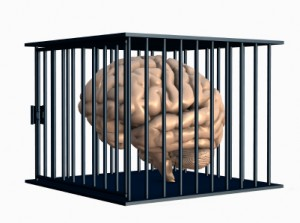
\includegraphics[width=1.0\textwidth]{KC.jpg}

\end{frame}

%%%%%%%%%%%%%%%%%%%%%%%%%%%%%%%%%%%%%%

\begin{frame}

\frametitle{Drasil}
\begin{center}
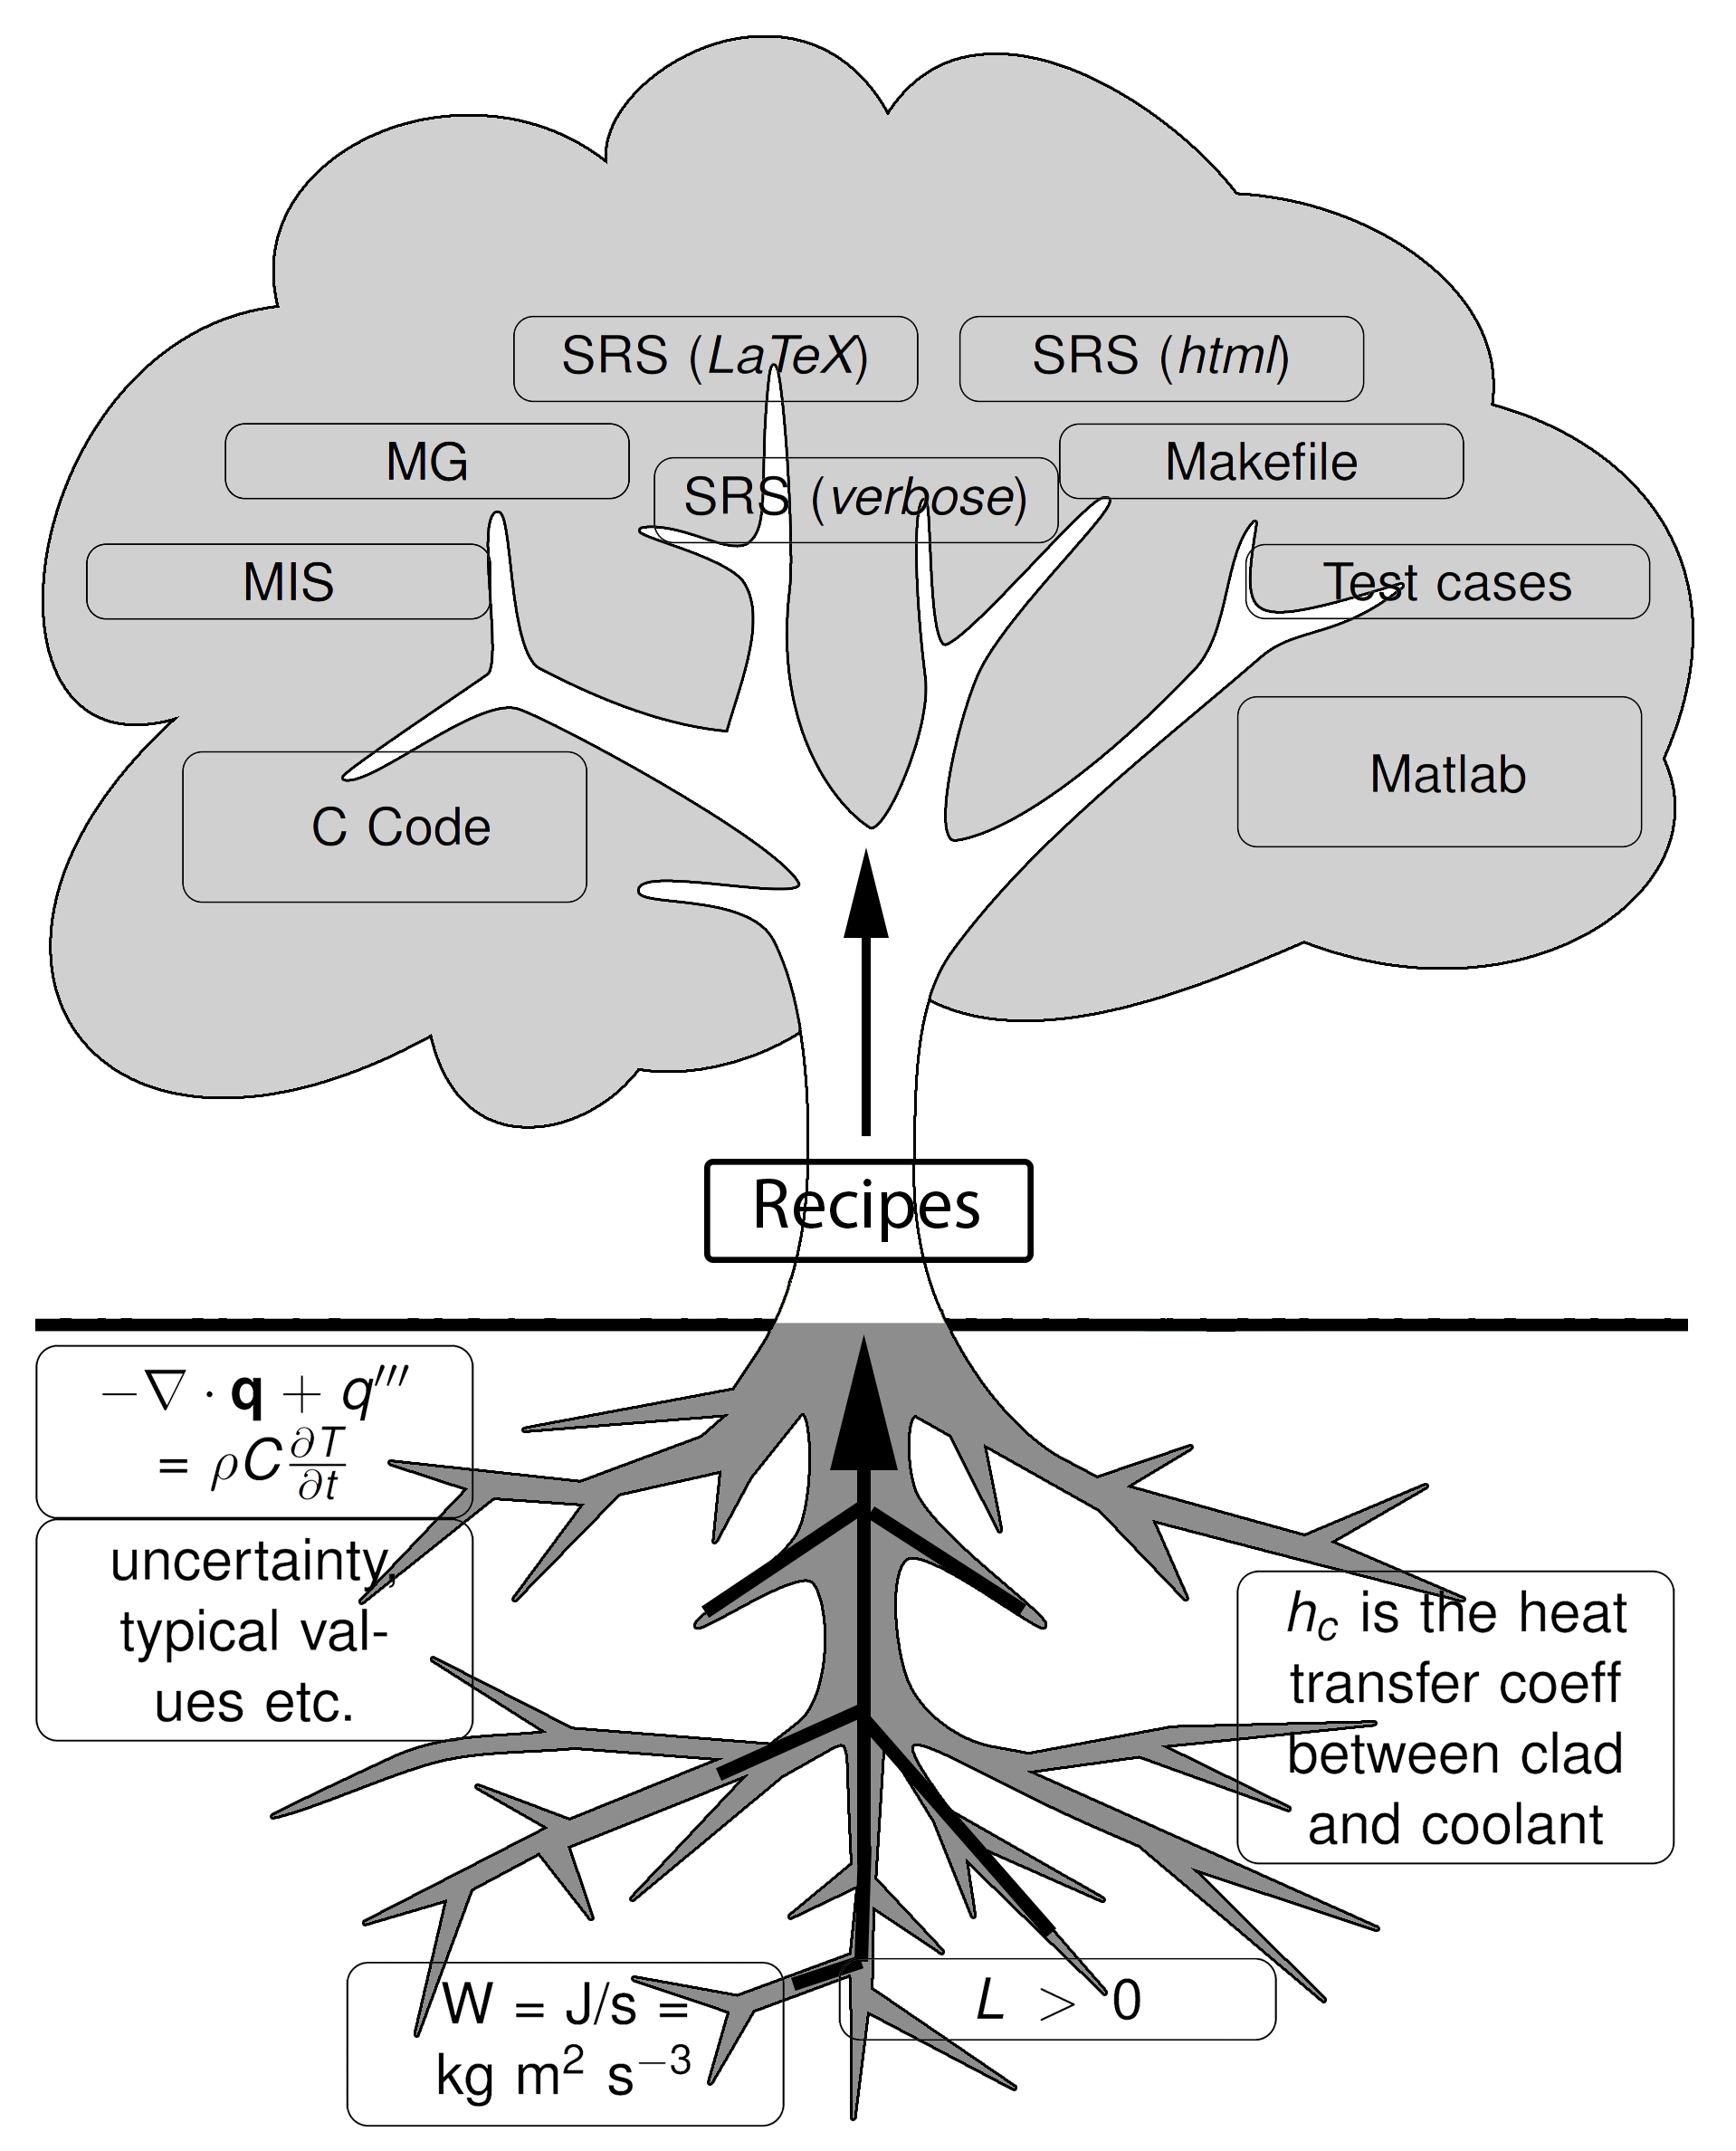
\includegraphics[height=21em]{tree.png}
\end{center}
\end{frame}

%%%%%%%%%%%%%%%%%%%%%%%%%%%%%%%%%%%%%

\begin{frame}

\includegraphics[width=\textwidth]{no_silver_bullet.jpg}
\end{frame}

%%%%%%%%%%%%%%%%%%%%%%%%%%%%%%%%%%%%%

% \begin{frame}

% \frametitle{Knowledge Based Approach}

% \begin{itemize}
% \item Capture knowledge
% \item From one ``source'' recipes to generate artifacts
% \item Automated
% \item Inspired by Knuth's Literate Programming
% \end{itemize}
% \end{frame}

%%%%%%%%%%%%%%%%%%%%%%%%%%%%%%%%%%%%%%

\begin{frame}

\frametitle{Advantages of Drasil}

\begin{itemize}
\item Supports changing requirements and design
\begin{itemize}
\item Generation
\item Automated traceability
\end{itemize}
\item Supports duplication 
\begin{itemize}
\item Knowledge is entered once, generated/transformed% as required
\item Eases maintenance
\item If incorrect, incorrect everywhere
\end{itemize}
\item Non-executable artifacts are generated
\end{itemize}
\end{frame}

%%%%%%%%%%%%%%%%%%%%%%%%%%%%%%%%%%%%%%

\begin{frame}
\frametitle{Design}

Drasil is currently being implemented as a combination of six eDSLs:

\begin{itemize}
\item Expression
\item Expression Layout
\item Document Layout
\item C Representation
\item \LaTeX{} Representation
\item HTML Representation
\end{itemize}

\end{frame}

%%%%%%%%%%%%%%%%%%%%%%%%%%%%%%%%%%%%%

\begin{frame}

\frametitle{Chunks}

\begin{center}
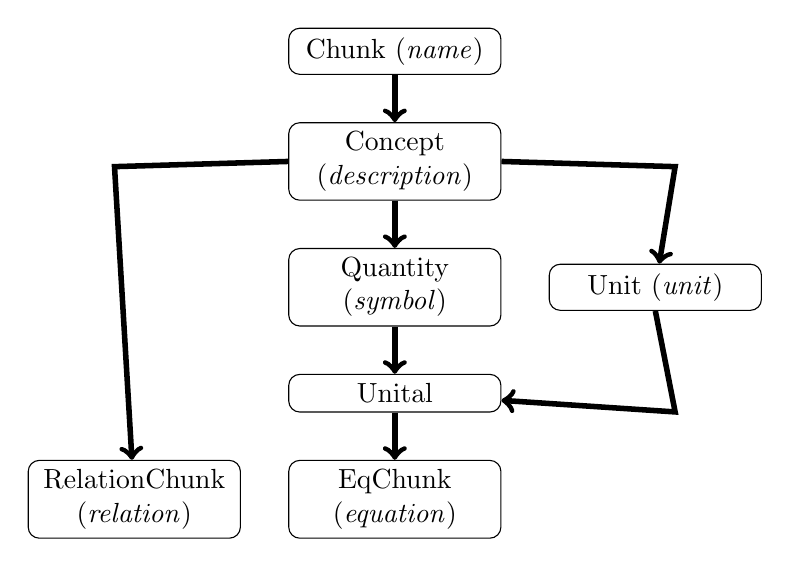
\begin{tikzpicture}[node distance=6mm]
  \tikzstyle{every node}=[draw,shape=rectangle, rounded corners,
    text width=7em, text centered];
  \node (ch)                     	{Chunk (\emph{name})};
  \node (co) [below = of ch]       {Concept (\emph{description})};
  \node (qu) [below = of co]  		{Quantity (\emph{symbol})};
  \node (u ) [right = of qu] 		{Unit (\emph{unit})};
  \node (uc) [below = of qu] 		{Unital};
  \node (eq) [below = of uc]	{EqChunk (\emph{equation})};
  \node (rc) [left = of eq]	{RelationChunk (\emph{relation})};

  \draw [->, line width=2pt] (ch) -- (co);
  \draw [->, line width=2pt] (co.west) -- (-3.56,-1.465) -- (rc); 
		%No idea how to do this
  \draw [->, line width=2pt] (co) -- (qu);
  \draw [->, line width=2pt] (co.east) -- (3.56,-1.465) -- (u );
  \draw [->, line width=2pt] (qu) -- (uc);
  \draw [->, line width=2pt] (u .south) -- (3.56,-4.58) -- (uc);
  \draw [->, line width=2pt] (uc) -- (eq);
\end{tikzpicture}
\end{center}

\end{frame}

%%%%%%%%%%%%%%%%%%%%%%%%%%%%%%%%%%%%%%

\subsection[Example]{Example}

%%%%%%%%%%%%%%%%%%%%%%%%%%%%%%%%%%%%%%

\begin{frame}[fragile]

\frametitle{Simple SRS from LaTeX}

\href{run:SRS.pdf}{SRS from LaTeX}\\
{SRS in HTML}

\end{frame}

%%%%%%%%%%%%%%%%%%%%%%%%%%%%%%%%%%%%%%

\subsection[Code]{Sample Code}

%%%%%%%%%%%%%%%%%%%%%%%%%%%%%%%%%%%%%%

\hoffset=-.5in %removing side bar for these frames

\begin{frame}[plain, fragile]

%\frametitle{Example Recipe}

\begin{lstlisting}
vars :: [EqChunk]
vars = [h_g, h_c]

s1, s2, s3, s4 :: LayoutObj
s1=table_of_units si_units
s2=table_of_symbols vars
s3=Section 0 (S "Data Definitions") $ map (Definition.Data) vars
s4=Section 0 (S "Code") $ map (CodeBlock.toCode CLang Calc) [h_c]

srs :: Quantity s => [s] -> String -> [LayoutObj] -> Document
srs ls author body =
  Document ((S "SRS for ") :+: 
    (foldr1 (:+:) (intersperse (S " and ") 
    (map (\x -> U $ x ^. symbol) ls))))
    (S author) body  
  
srsBody :: Document
srsBody = srs vars "Spencer Smith" [s1, s2, s3, s4]
\end{lstlisting}
\end{frame}

\hoffset=0in %resetting side bar
%%%%%%%%%%%%%%%%%%%%%%%%%%%%%%%%%%%%%%

\hoffset=-.5in %removing side bar for these frames

\begin{frame}[plain, fragile]

%\frametitle{Example Recipe}

\begin{lstlisting}

table_of_symbols :: (Unit s, Quantity s) => [s] -> LayoutObj
table_of_symbols ls=Section 0 (S "Table of Sym") [intro,table ls]

intro :: LayoutObj
intro = Paragraph $ 
  S "The table that follows ..."
  
table :: (Unit s, Quantity s) => [s] -> LayoutObj
table ls=Table [S "Symbol",S "Description",S "Units"] (mkTable
  [(\ch -> U (ch ^. symbol)), 
   (\ch -> ch ^. descr), 
   (\ch -> Sy $ ch ^. unit)] ls)
  (S "Table of Symbols") False

\end{lstlisting}
\end{frame}

\hoffset=0in %resetting side bar
%%%%%%%%%%%%%%%%%%%%%%%%%%%%%%%%%%%%%%

\hoffset=-.5in %removing side bar for these frames

\begin{frame}[plain, fragile]

%\frametitle{Example Recipe}

\begin{lstlisting}

fundamentals :: [FundUnit]
fundamentals = [metre, kilogram, second, ...]

derived :: [DerUChunk]
derived = [centigrade, joule, watt, calorie, kilowatt]

si_units :: [UnitDefn]
si_units = map UU fundamentals ++ map UU derived

------------- Fundamental SI Units ---------------------------------------------
fund :: String -> String -> String -> FundUnit
fund nam desc sym = UD (CC nam (S desc)) (UName $ Atomic sym)

metre, kilogram, second, ... :: FundUnit
metre    = fund "Metre"    "length"               "m"
kilogram = fund "Kilogram" "mass"                 "kg"
second   = fund "Second"   "time"                 "s"
kelvin   = fund "Kelvin"   "temperature"          "K"
mole     = fund "Mole"     "amount of substance"  "mol"
ampere   = fund "Ampere"   "electric current"     "A"
candela  = fund "Candela"  "luminous intensity"   "cd"

\end{lstlisting}
\end{frame}

\hoffset=0in %resetting side bar

%%%%%%%%%%%%%%%%%%%%%%%%%%%%%%%%%%%%%%

\hoffset=-0.5in %no side bar
\begin{frame}[plain, fragile]

%\frametitle{The $h_c$ Chunk}

$$h_{c} = \frac{2k_{c} h_{b}}{2k_{c}+\tau_{c}h_{b}}$$

\begin{lstlisting}

heat_transfer :: DerUChunk
heat_transfer = DUC (UD ht_con ht_symb) heat_transfer_eqn

ht_con :: ConceptChunk
ht_con = makeCC "Heat transfer" "Heat transfer"

ht_symb :: USymb
ht_symb = from_udefn heat_transfer_eqn

heat_transfer_eqn = USynonym (UProd 
  [kilogram ^. unit, UPow (second ^. unit) (-3),
   UPow (centigrade ^. unit) (-1)])

h_c_eq :: Expr
h_c_eq = 2*(C k_c)*(C h_b)/(2*(C k_c)+(C tau_c)*(C h_b))

h_c :: EqChunk
h_c = fromEqn "h_c" (S "convective heat transfer ...") 
  (lH `sub` lC) heat_transfer h_c_eq

\end{lstlisting}

\end{frame}

\hoffset=0in %resetting side bar

%%%%%%%%%%%%%%%%%%%%%%%%%%%%%%%%%%%%%%

\begin{frame}

\frametitle{Approach to Developing Drasil}

\begin{itemize}
\item Case studies
\begin{itemize}
\item Solar water heating tank
\item Slope stability analysis
\item Glass safety analysis
\item Game physics engine
\end{itemize}
\item Practical
\item Not trying to automate everything %trust developer
\item Small chunks of knowledge
\item Look for patterns
\item Tool support
\begin{itemize}
\item Version control
\item Issue tracking
\item Regression testing
\end{itemize}
\end{itemize}

\end{frame}

%%%%%%%%%%%%%%%%%%%%%%%%%%%%%%%%%%%%%%

\hoffset=-0.4in %no side bar
\begin{frame}[plain, fragile]

\frametitle{Refactor}

\begin{lstlisting}

boiling = makeCC "Boiling" 
  "Phase change from liquid to vapour"
phsChgMtrl  = makeCC "PCM" "Phase Change Material"
liquid  = makeCC "Liquid" "liquid state"
solid   = makeCC "Solid" "solid state"

...

Paragraph (S "This derivation does not consider the " :+: 
(sMap (map toLower) (S (boiling ^. name))) :+: S " of the " :+: 
S (phsChgMtrl ^. name) :+: S ", as the " :+: S (phsChgMtrl ^. 
name) :+: S " is assumed to either be in" :+: S " a " :+:
(solid ^. descr) :+: S " or a " :+: (liquid ^. descr) :+: 
S " (A18).")]

\end{lstlisting}

\end{frame}

\hoffset=0in %resetting side bar

%%%%%%%%%%%%%%%%%%%%%%%%%%%%%%%%%%%%%%

\section[Future Work]{Future Work}

%%%%%%%%%%%%%%%%%%%%%%%%%%%%%%%%%%%%%%

\begin{frame}

\frametitle{Future Work}

\begin{itemize}
\item Cleaner separation between knowledge and recipes
\item Generate additional software artifacts
\item Capture design decisions
\item Develop alternative recipes
\item Assurance case for FMRI statistical correlation
\item Predict solid fraction for metal alloy cooling
\item Testing
\begin{itemize}
\item Guards on input
\item Sanity checks
\item Metamorphic testing
\item Computational variabilty testing
\end{itemize}
\end{itemize}

\end{frame}

%%%%%%%%%%%%%%%%%%%%%%%%%%%%%%%%%%%%%%

\section[Conclusions]{Conclusions}

%%%%%%%%%%%%%%%%%%%%%%%%%%%%%%%%%%%%%%

\begin{frame}

\frametitle{Drasil Framework for LSS}

\begin{itemize}
\item SCS has the opportunity to lead other software fields%  by leveraging its
  % solid existing knowledge base
\item Document driven design is feasible% with a knowledge-based approach
\item Requires an investment of time %to build knowledge base
\item Documentation does not have to be painful
\item Develop/refactor via practical case studies
\item Ontology may naturally emerge
\end{itemize}


\includegraphics[width=0.5\textwidth]{../WG2_11/generate_all_the_things.jpg}

\begin{tikzpicture}[remember picture,overlay]
\node [xshift=2.75cm,yshift=-2.15cm] at (current page.center)
{
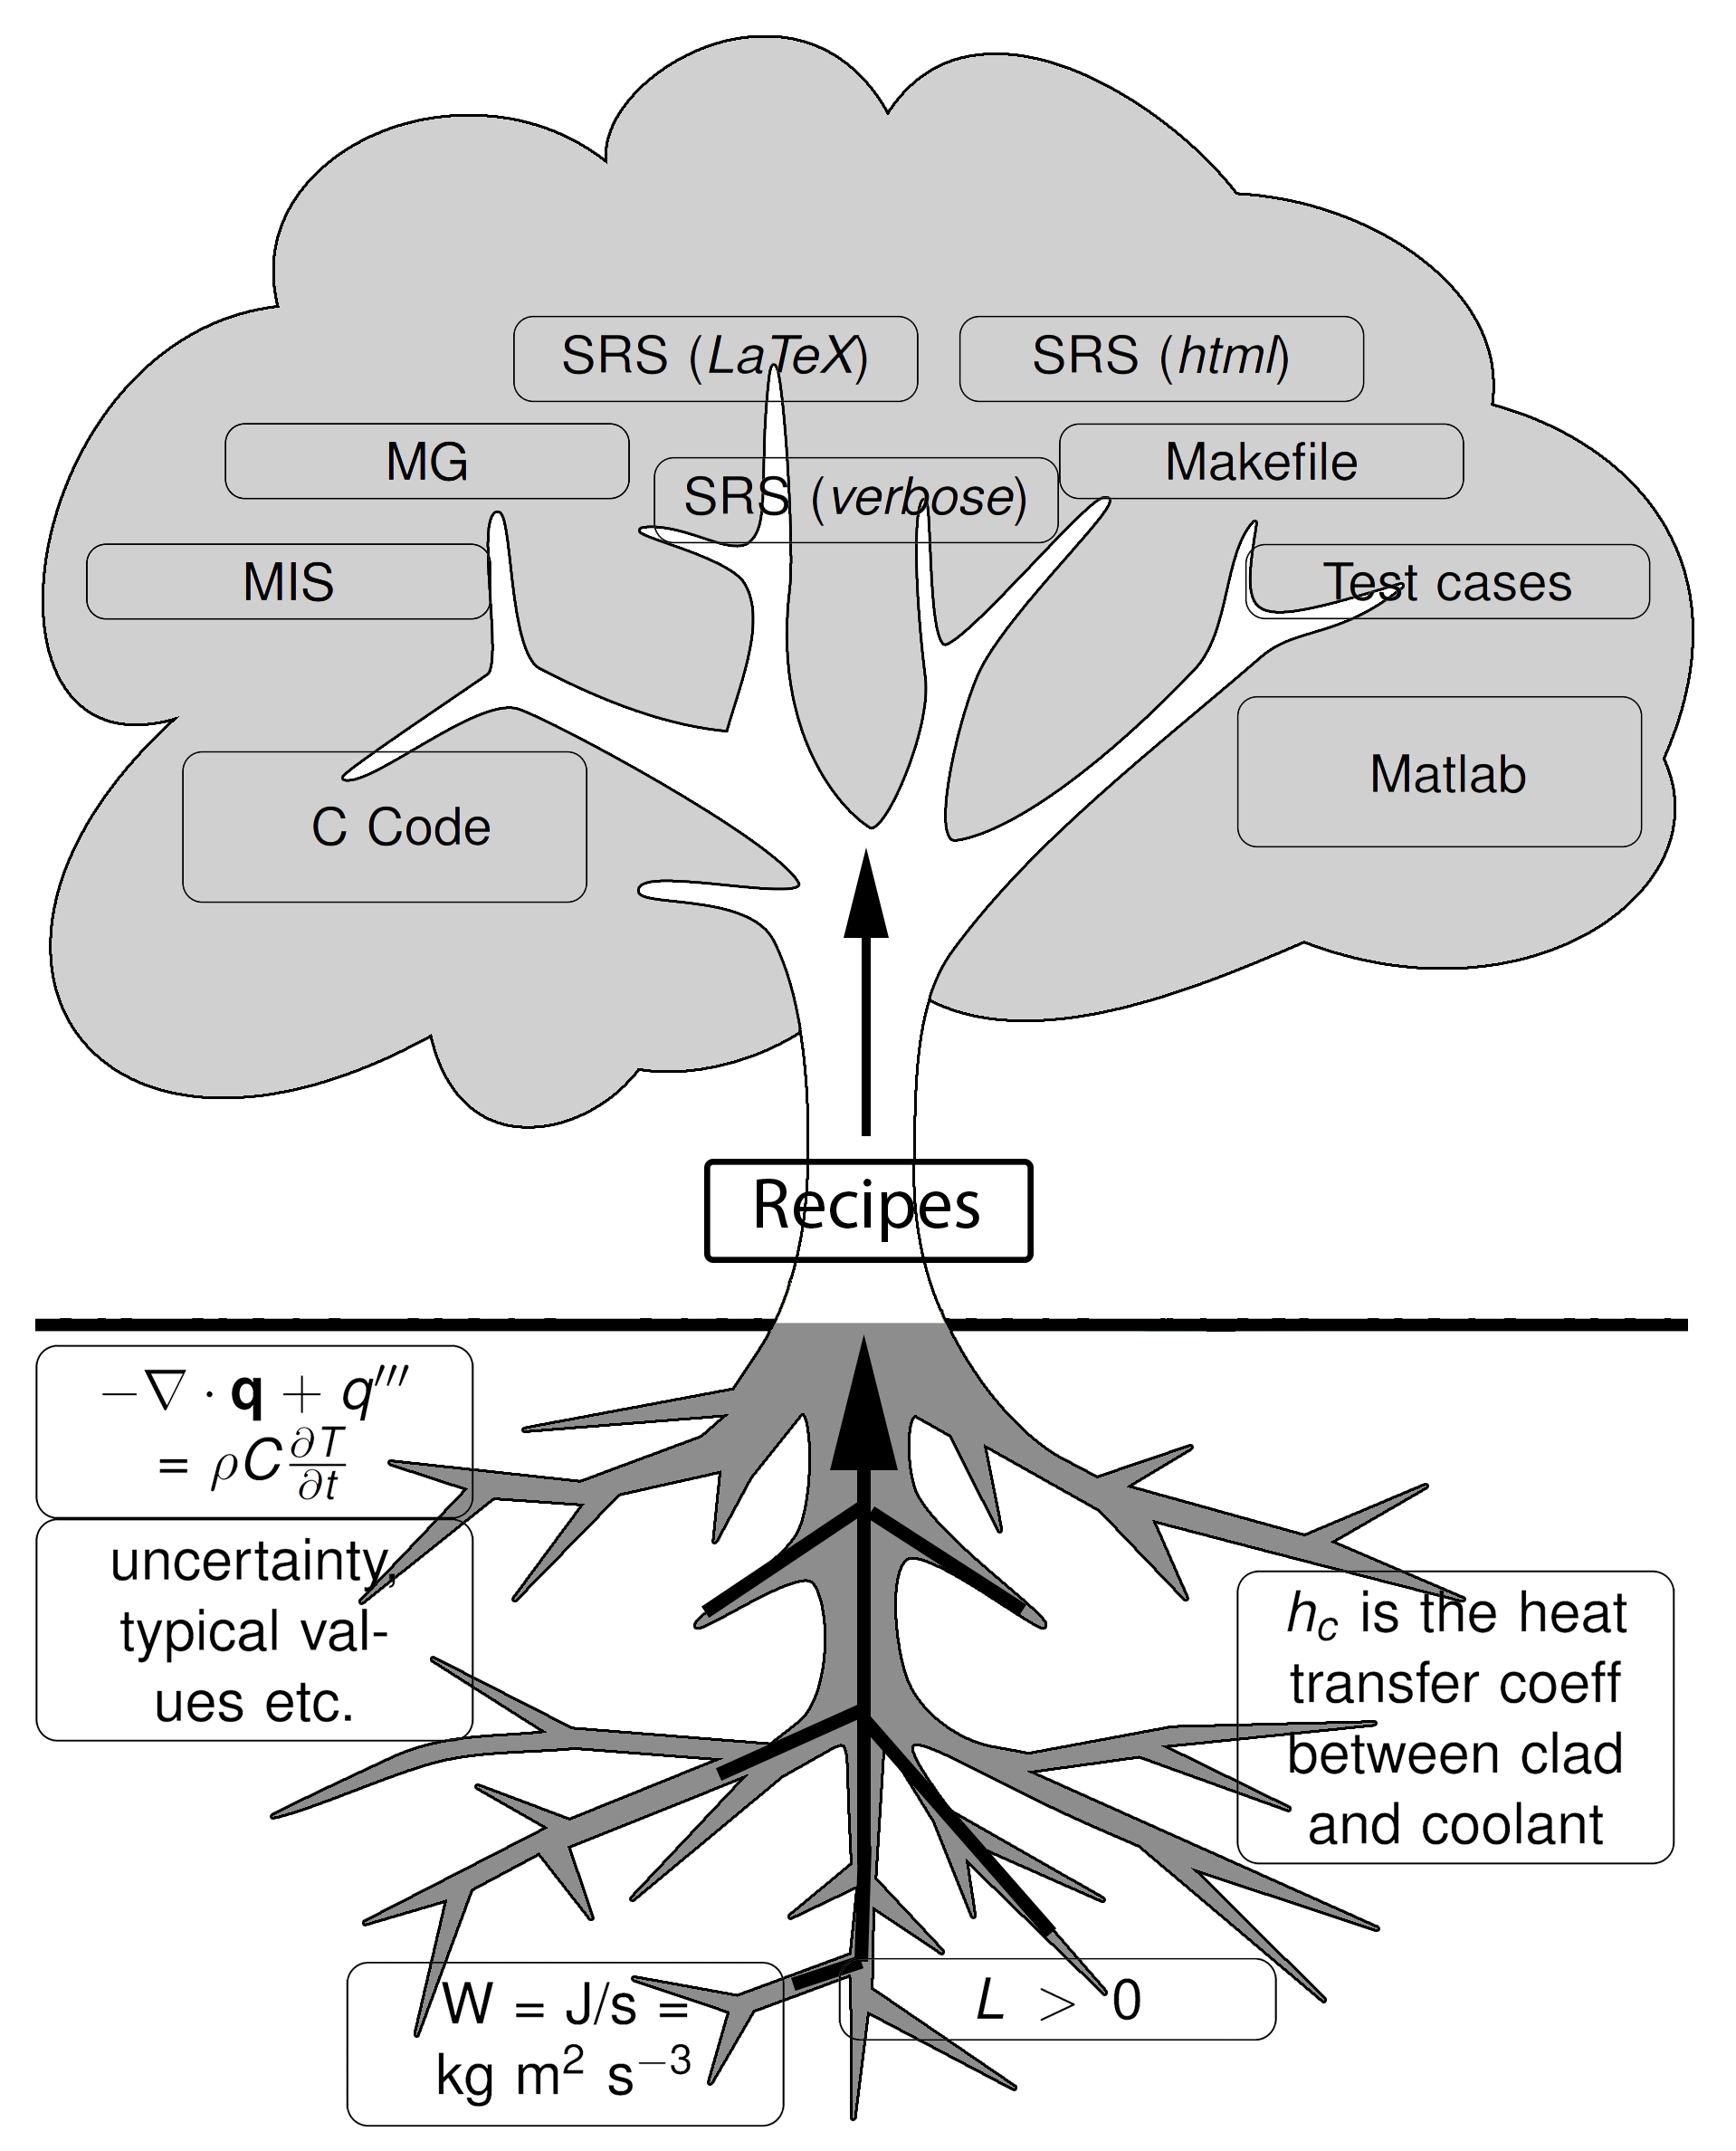
\includegraphics[height=10em]{tree.png}
};
\end{tikzpicture}

\end{frame}

%%%%%%%%%%%%%%%%%%%%%%%%%%%%%%%%%%%%%%

% \begin{frame}

% \frametitle{Acknowledgements}

% \begin{itemize}
% \item Jacques Carette
% \item Dan Szymczak
% \item Steven Palmer
% \item ...
% \end{itemize}
% \end{frame}

%%%%%%%%%%%%%%%%%%%%%%%%%%%%%%%%%%%%%%

\begin{frame}[allowframebreaks]
\frametitle{References}
\bibliography{CSE_2016}
\bibliographystyle{plainnat}
\end{frame}

%%%%%%%%%%%%%%%%%%%%%%%%%%%%%%%%%%%%%%

\end{document}